%
% Demo doc that tests most of the features of the cu-thesis class
% This version tests the 'final' option, which generates a PDF/A file for submission
%
% NOTE: if cu-thesis is installed on your system, documentclass can just be cu-thesis
%
\documentclass[ %% Final will produce PDF/A for submission
    final,
    scrbook,
    listoffigures,
    listoftables, 
    glossary]{cu-thesis}

% Packages for this test doc to generate text and verify figures
% you probably don't want these
\usepackage{blindtext}
\usepackage{lipsum}

\usepackage{geometry}
\geometry{left=1in, right=1in, top=1in, bottom=1in}


%\usepackage[demo]{graphicx}
\usepackage{caption}
\usepackage{subcaption}

% percent Useful packages
\usepackage{amsmath}
\usepackage{amsfonts}

\usepackage{graphicx}
\usepackage[colorlinks=true, allcolors=blue]{hyperref}
\usepackage{color,soul}
\newtheorem{theorem}{Theorem}[section]
\newtheorem{corollary}{Corollary}[theorem]
\newtheorem{lemma}[theorem]{Lemma}
\newenvironment{proof}[1][Proof]{\par\noindent\textit{#1.} }{\hfill $\square$\par}
\DeclareMathOperator*{\argmax}{argmax}

\usepackage{array}
\usepackage{multirow}
\usepackage{tabularx}
\usepackage{longtable}
%\usepackage[showframe]{geometry}

\usepackage{natbib}
\usepackage{booktabs} 
%\usepackage[utf8]{inputenc}
%\usepackage{afterpage}
\usepackage{float}
%\usepackage[showframe=true]{geometry}
%\usepackage{changepage}

\usepackage{listings}
\usepackage{xcolor}

\definecolor{codegreen}{rgb}{0,0.6,0}
\definecolor{codegray}{rgb}{0.5,0.5,0.5}
\definecolor{codepurple}{rgb}{0.58,0,0.82}
\definecolor{backcolour}{rgb}{0.95,0.95,0.92}

\lstdefinestyle{mystyle}{
    backgroundcolor=\color{backcolour},   
    commentstyle=\color{codegreen},
    keywordstyle=\color{magenta},
    numberstyle=\tiny\color{codegray},
    stringstyle=\color{codepurple},
    basicstyle=\ttfamily\footnotesize,
    breakatwhitespace=false,         
    breaklines=true,                 
    captionpos=b,                    
    keepspaces=true,                 
    numbers=left,                    
    numbersep=5pt,                  
    showspaces=false,                
    showstringspaces=false,
    showtabs=false,                  
    tabsize=2
}

% Set up bibtex or biblatex here
%\usepackage{cite}
\usepackage{layout}
%\renewcommand{\thesection}{\Alph{section}}

% SETUP: Document Details
\title{Aging Impact on Unemployment - a Price Adjustment Mechanism}
\author{Fuguang Chen}
\date{February 2024}

% The title page uses the following options to piece together the subject line 
% "A [thesistype] submitted to [submitted to] in partial fullfilment of ... etc
\thesistype{thesis proposal}
\submittedto{the thesis proposal committee}
\degree{Master of Computer Science}
\program{Degree Program}
\submissiondate{2024}

% Abstract, acknowledgements
\abstract{This thesis investigates the influence of aging on the labor market, specifically focusing on its impact on unemployment and the prices of goods. The analysis is grounded in a collection of empirical observations from different countries, revealing a noteworthy trend: retired individuals not only exhibit reduced consumption expenditures compared to working individuals, but also tend to purchase the same goods at lower prices.

To understand this phenomenon, two different models are created: one is a conventional mathematical search-matching model, and the other is an agent-based model. These models offer insights into the underlying mechanism that enables retired seniors to access more affordable goods, as they possess increased time for thorough searches in the product market. 

We find two interesting and opposing effects: Initially, the growing population of retirees amplifies net demand, thereby stimulating employment opportunities. Simultaneously, however, the retirees have higher price sensitivity, compelling firms to maintain competitive pricing. This, in turn, erodes corporate market power, diminishes profit margins, and deters incentives for employment generation. Paradoxically, this increased demand results in lower profits for firms and higher unemployment rates.  Finally, we show that our models exhibits similar qualitative trends as data from the World Bank's World Development Indicators, and offers a way of reconciling predictions on the economic impact of aging populations.

%\vspace{\baselineskip}
%    \noindent \textbf{Keywords:} Old-age Dependency Ratio, Unemployment Rate, Labor Market Tightness, Search Intensity
}
\acknowledgements{Reflecting on the journey that has led to this thesis, I am filled with gratitude for the many individuals whose support has been essential to my academic and personal growth. At the forefront is my advisor, Alan Tsang. His steady commitment to academic excellence, attention to detail, and patience with the mistakes I've made have been crucial in guiding me through this challenging process. Alan's enthusiasm for research is inspiring, and his valuable advice has been a guiding light in completing this journey. Without his guidance, I can't imagine reaching this milestone. To Alan, I offer my deepest thanks for his mentorship and faith in my abilities.

To my parents, I owe you so much. Words cannot fully express my deep appreciation for your unconditional love and support. Even knowing you wouldn't see your son in person for more than five years, you've stood by my side without hesitation. Your sacrifices have allowed me to pursue my academic dreams far from our home. The strength and encouragement you've given me have been the foundation of my persistence. This thesis is dedicated to you, as a token of my deep appreciation and love.

Last but certainly not least, a heartfelt thank you to my wife and our children, Huanyan and Maoxiu. Your love and presence have made me a more peaceful and grounded person. The joy and stability you bring to my life have been my sanctuary. Thank you for being my constant source of happiness and for making our house a home.}

% PDF meta-info:
\subjectline{\@title}
\keywords{keyword 1, keyword 2, etc.}

\begin{document}
    % Create the frontmatter (title page, abstract, toc, etc.)
    \frontmatter
%\usepackage[utf8]{inputenc}

\chapter{Introduction}
Since the beginning of the 21st century, aging becomes a more serious issue in many countries. In two decades after 2000, the proportion of the population over 65 years old increased from 12.49 percent to 18.52 percent in Canada\footnote{Data Source: World Development Indicators, World Bank as of May 10, 2023}.
\begin{figure}[h]
\centering
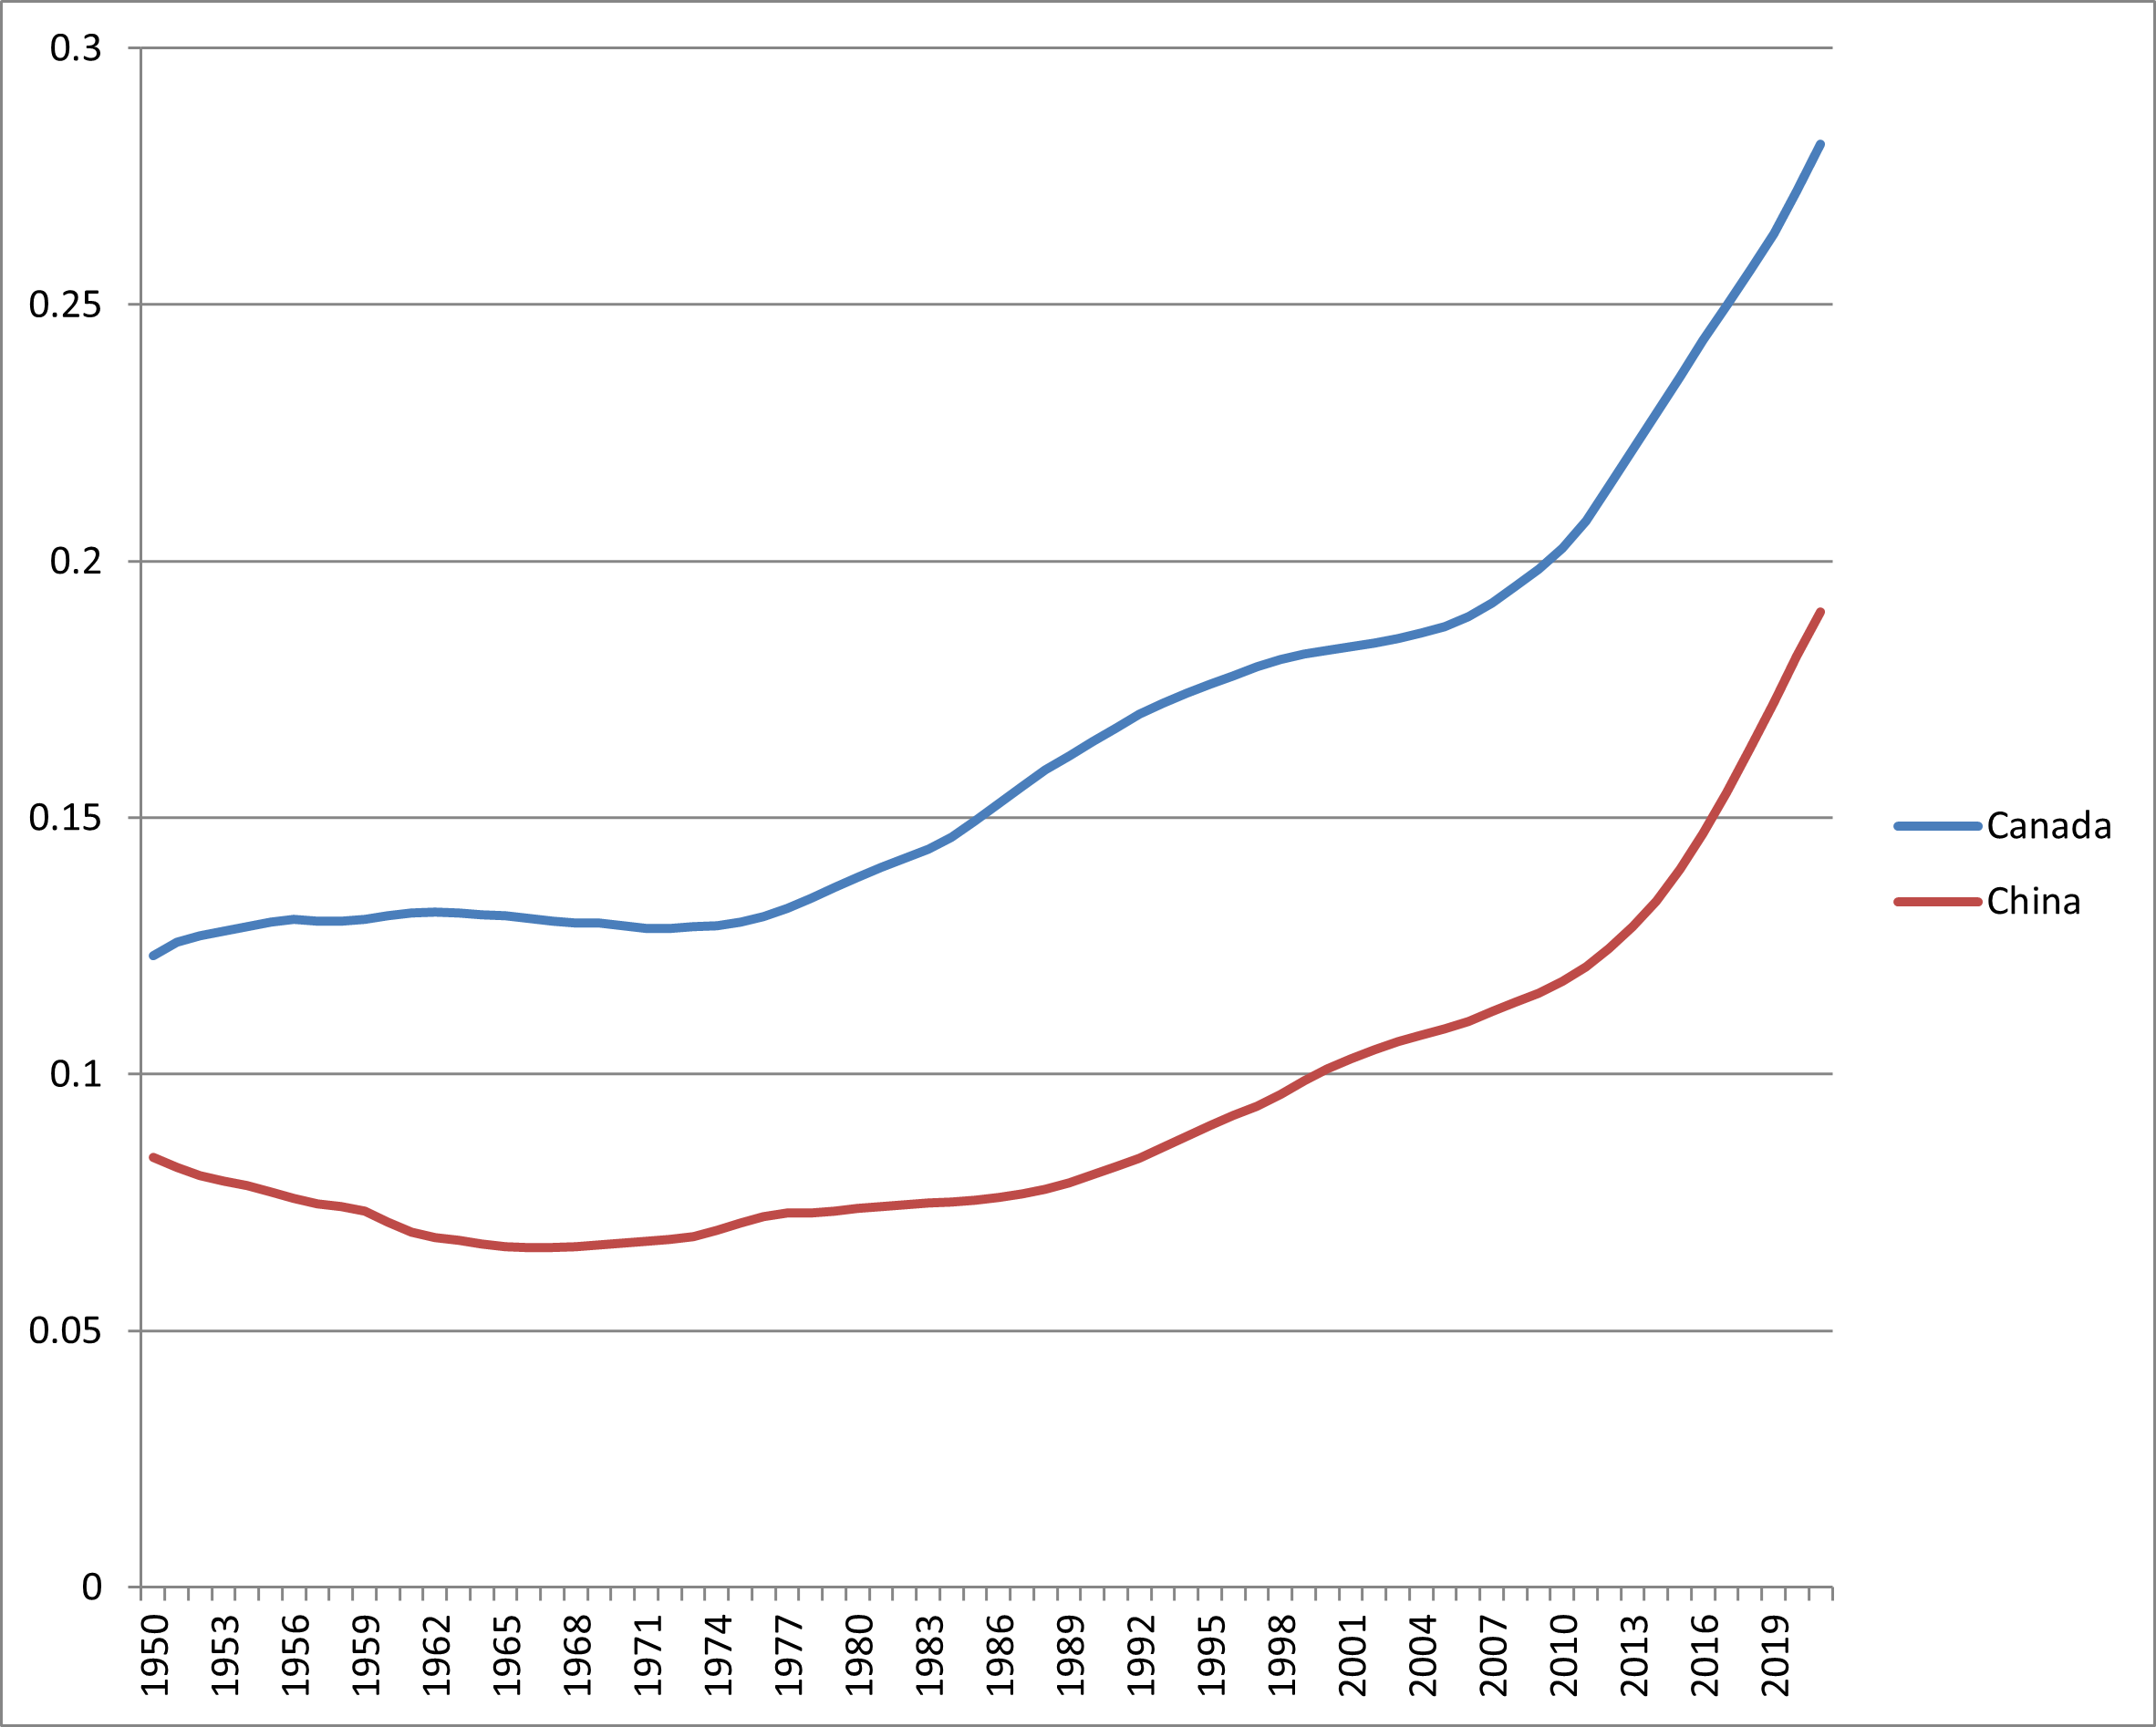
\includegraphics[width=10cm, height=8cm]{population trend.png}
\caption{The Proportion of the Population over 65 years old in Canada and China}
\end{figure}
To understand the impact of these trends, we must answer several questions: Is population aging good for firms' profit? What impact will aging have on per capita consumption and income? An equivalent question would be: what impact does aging have on productivity growth? The main work of this paper is to consider the impact of demographic changes on macroeconomic variables, especially the labor market. A key measurement of a population's age distribution is the {\textbf old-age dependency ratio}, which is the ratio of number of working individuals to the number of retirees.  A low old-age dependency ratio means there are many workers supporting each retiree; While a high ratio indicates economic troubles caused by few workers supporting each retiree. Take Japan, one of most aged countries in the world, for example, the value is 0.51 in 2022\footnote{Data source: https://wdi.worldbank.org/table/2.1}, which means means a group of 100 working individuals needs to support 51 retirees who are no longer working. 

In this paper, to simulate the empirical environment, we introduce a conventional search and matching mathematical model, and an agent-based model of the economics of an aging population, followed by a comparison of the results with real world data. Our main innovation is the introduction of search intensity into the analysis of labor market; that is, shoppers in different ages show different time use for even identical goods. In our model, the concept of search intensity among shoppers in the goods market can be defined by a value that represents the likelihood of a shopper deciding to conduct further searches after an initial encounter with a seller. For example, a search intensity value of 0.9 indicates that there is a 90\% probability that a shopper will engage in a second search for goods after meeting with a seller. A higher value signifies that a shopper is likely to spend more time searching, reflecting a greater degree of search behavior in her purchasing process. Our findings provide a new perspective for macroeconomic analysis from an aging perspective. The introduction of unemployment is first and foremost because employment is also one of the core concerns of policymakers in countries with aging populations. 
Our contribution is to propose a mathematical and an agent-based framework to analyze the transition mechanism between the aging and labor market. 

\chapter{Related work}
\section{Aging and Unemployment}
After residents retire, consumption will decline \cite{hamermesh1980unemployment}. Taking the UK as an example, residents significantly reduce consumption after retirement, and this reduction cannot be explained by the life cycle model \cite{banks2006retirement}. Data from the United States also supports this view. Bernheim et al. \cite{bernheim2001accounts} ’s study of panel data on household income dynamics in the United States shows that the elderly reduce consumption after retirement. This is the so-called “retirement-consumption puzzle.” Population aging will have an impact on the consumption of the elderly and the demand structure of the entire society. Certain economic sectors, such as the medical and food sectors serving the elderly, will expand significantly relative to sectors such as education, transportation and housing services \cite{hagemann1989population}. Thießen \cite{thiessen2007aging} believe that the above-mentioned industry changes may increase the cross-industry flow of employed people. When most employees newly entering the industry are relatively unskilled, this flow will in turn lead to labor productivity, at least in the short term, decline. Through an empirical analysis of household data from the Austrian Consumer Budget Survey, Aigner-Walder and D\"{o}ring \cite{aigner2012effects} found that the increase in the proportion of the elderly population will lead to a decrease in the consumption of goods and services in the transportation sector, while health products and services consumption of housing, water, electricity, coal and other fuels, food and nonalcoholic beverages will rise. The same conclusion can be found using data from the US Panel Study of Income Dynamics. If the owner of a household suddenly loses his job, the consumption of daily necessities such as food will decrease by about 15\% \cite{stephens2002worker}. 

There are several channels that aging changes consumption and then affects investment, savings and employment: the decline in per capita consumption may be because the rise in aging will hinder the increase in labor participation rate \cite{sheiner2007primer}; aging can also change people’s consumption pattern, further leading to a decline in the consumption of the elderly \cite{banks2006retirement}; the decline in expenditures of the elderly is also possible. It is due to the substitution effect between consumption and leisure time \cite{hurd2003retirement}. Hock et al. \cite{hock2012dynamics} used a
continuous time intertemporal substitution model based on the impact of population aging caused by declining birth rates and prolonged life expectancy on consumption, and believed that the decline in consumption caused by longer life expectancy may be solved by increasing the birth rate.

Although the analysis of the impact of aging on the macro economy has also started from the supply side \cite{maestas2023effect}, most analysis still emphasizes the impact of aging on the demand side of the economy, because the transformation in the demographic composition, particularly the age distribution within a population, will inevitably lead to a shift in consumer preferences and the types of goods and services demanded. Consequently, this alteration in demand will significantly influence the distribution of employment opportunities across various economic sectors, as industries adapt to cater to the changing needs and consumption patterns of the population~\cite{borsch2003labor}. This change is confirmed by Fougere et al. \cite{fougere2007sectoral}, Luhrmann \cite{luhrmann2008effects} and Rausch \cite{rausch2009macroeconomic}. Empirically, Katagiri \cite{katagiri2020aging} used the classic search matching theory to analyze the impact of aging in Japan. By establishing a multi-sector New Keynesian model, he found that aging caused 0.3\% deflationary pressure on Japan from 1990 to 2000, ranging from 0.3\% to 0.4\% rise in structural unemployment.

\section{Shopping Behaviors by Age}
\label{shopping_by_age}
When establishing a micro-foundation and putting the theory of population aging and unemployment into a unified analytical framework, many literature ignore the fact that the retirees have more time: they have more time to shop around, and they can find products of the same quality but at a lower price, or products of the same price but with higher quality. In other words, the retirees have stronger search intensity and higher bargaining power with manufacturers/sellers. Aguiar et al. \cite{aguiar2007life} used the data of the American ``AC Nielsen's Homescan Survey'' (ACNielsen's Homescan Survey) to find that for the same goods, the average price paid by households whose head is in their 40s is more than 4 percent higher than that of households over 65. 

Despite the increasing size of the aging population, research on its consumption behavior has not received due attention. At present, most of the literature is launched from the perspective of marketing to the retirees. Swinyard et al. \cite{swinyard1994six} examined the factors influencing the preferences of American "Baby Boomers" for discount store shopping and explored the diversity in shopping characteristics and price sensitivity among this older consumer demographic through sample questionnaires. Moschis et al. \cite{moschis1997targeting} described corporate stereotypes of older consumers: poorer health and dissociated from the general public; Szmigin et al. \cite{szmigin2001learning} and Myers et al. \cite{myers2008understanding} explored the conservative and penny-pinching spending habits of the aged shoppers. Hawes et al. \cite{hawes1984understanding} studied the market behavior of elderly consumers and investigated the impact of retirement on the consumption behavior of the retirees. The findings suggest that age, not retirement, is a key factor in older adults' shopping behavior. 


%Kaplan and Menzio (2016)~\cite{kaplan2016shopping} makes use of this assumption in their shopping behavior model.
%Interestingly, similar to unemployed workers, senior shopping shares several similar characteristics. 


\iffalse
Source:  Statistical Survey Department, Statistics Bureau, Ministry of Internal Affairs and Communications.
Consumer Expenditure Surveys, https://www.bls.gov/cex/tables/calendar-year/mean-item-share-average-standard-error.htm
\fi


\section{Agent-based Modeling}
Agent-Based Modeling (ABM) has emerged as a powerful tool in understanding the complex dynamics of economic systems, particularly in the context of aging populations and their impacts on the goods and labor markets. Studies using ABM have made significant contributions to understanding how aging impacts markets. This highlights the versatility and depth of insights these models offer. Windrum et al. \cite{windrum2009consumer} provided an early foundation for using ABM in economic simulations, highlighting its potential to capture individual behaviors and market dynamics in ways traditional models cannot. Their work emphasized ABM's capacity to integrate heterogeneous agents and complex interactions, setting a precedent for subsequent studies on aging and economic dynamics. Silverman et al. \cite{silverman2013demography} explored how aging populations affect labor market dynamics through ABM. They modeled the workforce's aging process and examined the implications for productivity, unemployment, and job matching. Their findings suggested that an aging workforce could lead to increased skill mismatches and longer job search times, illuminating the nuanced ways in which demographic shifts impact labor markets. On the goods market side, Axtell \cite{axtell2016120} applied ABM to understand how aging populations influence consumption patterns and price dynamics. Their model incorporated consumer heterogeneity, including age-based preferences and income levels, to demonstrate how shifts in the age distribution could alter demand patterns, affecting price adjustments and market equilibrium.
\section{Search and Matching Model}
In context of theoretical framework of the model, Mortensen and Pissarides \cite{mortensen1994job} fundamentally changed our understanding of labor market dynamics through their Search and Matching Model, illustrating how unemployment and job vacancies persist simultaneously due to various labor market frictions, which refer to the various factors that prevent the labor market from clearing (that is, they hinder the efficient matching of job seekers with job vacancies). These frictions can result from information asymmetry between employers and job seekers, geographical mobility issues, and skills mismatch, all of which contribute to the inefficiency of the job matching process. Their model uses a matching function $M(U, V)$ to quantify how efficiently vacancies and unemployed workers pair up, considering the roles of both job seekers and employers in this process \cite{pissarides2000equilibrium}.
Additionally, the aging of the population introduces significant shifts in labor market dynamics, affecting both the supply and demand for labor. Autor et al. \cite{autor2013growth} discuss how demographic changes, particularly aging, impact labor market outcomes through alterations in the workforce composition. They argue that older workers face unique challenges, including longer durations of unemployment and potential discrimination, which can exacerbate the frictions outlined by the Search and Matching Model. Aging can influence the matching efficiency negatively, as older workers might have more difficulty finding suitable employment due to evolving industry demands and the potential skills obsolescence \cite{bhattacharya2001aging}.
About the impact of aging on unemployment rate, there are diverse results based on individual channel.
Considering unemployment rate of younger and senior workers,  Pissarides \cite{pissarides1989unemployment} and  Shimer \cite{shimer2001impact}
argue that the declines in the shares of teenagers and young adults in the labor force have put measurable downward pressure on unemployment rates, as younger workers have higher unemployment rate than the aged. This conclusion is confirmed by De la Croix et al. \cite{de2013aging} which elaborated a channel through which aging leads to lower interest rate, stimulating lower cost of labor demand for the firms.
However, Cociuba et al. \cite{cociuba2018demographics} takes the opposite view that a larger fraction of young workers at high population growth results in lower employment rates and lower population growth results in longer periods of high unemployment.

In context of empirical findings, research exploring the relationship between an aging workforce and unemployment rates presents a complex picture. For instance, Shimer \cite{shimer2005cyclical} found that demographic shifts, including aging, can lead to variations in the unemployment rate due to changes in job search behavior and retirement patterns. However, the effect is nuanced; while older workers may experience longer spells of unemployment \cite{kroft2016long}, the overall unemployment rate could be influenced by the labor force participation rate of this demographic group and their job acceptance rates, which could potentially lower the overall unemployment rate as they exit the workforce or accept positions more readily \cite{fallick2006job}.

Moreover, the application of the Search and Matching Model to assess the effectiveness of policy interventions aimed at reducing unemployment among older workers reveals varied outcomes. For example, policies such as retraining programs, subsidies for hiring older workers, and enhancements to job search assistance are designed to reduce the frictional unemployment specific to this group \cite{lalive2008impact}. These studies utilize the framework provided by the Search and Matching Model to evaluate how such interventions can improve the matching efficiency and potentially reduce the duration of unemployment for older workers.


%%%%%%%%%%%%%%%%%%%%%%%%%%%%%%%%%%%%%%%%%%%%%%%%%%%%%%%%%%%%%%%%%%%%%%%%
\iffalse
\chapter{}

When establishing a micro-foundation and putting the theory of population aging and unemployment into a unified analytical framework, many literature ignore the fact that the elderly have more time, they have more time to shop around, and they can find products of the same quality but at a lower price, or products of the same price but with higher quality. In other words, the elderly have stronger search intensity and higher bargaining power with manufacturers. If classified according to the shopping characteristics of buyers in the product market, it includes employed persons of the right age (i.e. those who are employed and aged between 16 and 64), unemployed persons of the right age (i.e. unemployed and looking for Works aged 16-64) and the elderly (i.e., retired people aged 65 and over who are no longer entering the labor force) differ in their search intensity. \cite{aguiar2007life} used the data of the American "AC Nielsen's Homescan Survey" (ACNielsen's Homescan Survey) to find that for the same goods, the average price paid by households whose head is in their 40s is more than 4 percent higher than that of households over 65. The elderly no longer need to participate in the labor market, so they start to have a lot of leisure time, and the cost of time is much lower than before retirement. Reflected in the goods market, they are more willing to use low-cost time to replace prices, and tend to spend more time looking for lower-priced goods. Despite the increasing size of the aging population, research on its consumption behavior has not received due attention. At present, most of the literature is launched from the perspective of marketing to the elderly.  et al.~\cite{swinyard1994six} analyzed the reasons why the American "Baby Boomers" prefer to shop in discount stores and the heterogeneity among older consumers through sample questionnaires. \cite{moschis1997targeting} described corporate stereotypes of older consumers: poorer health and dissociated from the general public; \cite{szmigin2001learning} and \cite{myers2008understanding} explored the Conservative and penny-pinching spending habits of the aged shoppers. \cite{hawes1984understanding} studied the market behavior of elderly consumers and investigated the impact of retirement on the consumption behavior of the elderly. The findings suggest that age, not retirement, is a key factor in older adults' shopping behavior. Differences between older and younger consumers are developed and suggestions for further research are provided.


\fi

\chapter{Search and Matching Model}
Accelerated demographic change will be one of the key factors shaping social development. Most of the literature on aging has focused on the implications of demographic trends for social policy, particularly pension balance issues~\cite{wacker2010aging,carta2021workforce,bongaarts2004population,vogel2017aging}. 
However, demographic changes will also trigger far-reaching structural changes at the macroeconomic level, which are further reflected in economic activities, such as labor markets, goods and services markets, and so on. 
%There are very few literature on the aging of the labor market. To the author's understanding,
Literature on aging of the labor market is abundant; however, most of them focuses on how changes in the age structure of the labor force affect the unemployment rate or labor force participation rate of young or old people~\cite{barnichon2018demographic,bell2011young,bhattacharya2001aging,johnson2012age}. Instead, we intend here to examine the effect that an aging workforce has on unemployment within the working age population.
Our approach is motivated by \cite{burdett1983equilibrium}. They recognize that searching the market for lower prices is time consuming, a limited resource for a worker, but one that is more available for the unemployed or retired.  As a result, these segments of the population exhibit increased price sensitivity and are generally better able to purchase goods at lower prices. Krueger et al.~\cite{krueger2010job} further show that unemployed people spend more time shopping and pay less for their goods than their employed counterparts. These motivate the analysis of Kaplan and Menzio~\cite{kaplan2016shopping}, where the unemployed and the employed behave very differently in goods markets. They show that unemployed people spend more time shopping and pay less for their goods. Interestingly, similar to unemployed workers, seniors’ shopping also has several similar characteristics. This is evident when examining data from the Survey
of Time Use of Americans (ATUS) data from 2003 to 2016, we find that older adults spend significantly more time shopping. Figure \ref{fig:ats} shows the trend of shopping time for different age groups. 
\begin{figure}[h]
\centering
\includegraphics[width=0.75\linewidth]{time use by age.png}
\caption{US Time Spent Shopping by Age}
\label{fig:ats}
\end{figure}

Moreover, even for the same goods, seniors pay lower prices~\cite{aguiar2007life}. The retirees no longer need to participate in the labor market, so they start to have a lot of leisure time, and the cost of time is much lower than before retirement. Reflected in the goods market, they are more willing to use low-cost time to replace prices, and tend to spend more time looking for lower-priced goods, which can be verified from the data shown in Figure 3.2.\footnote{Data Source:

\raggedright Statistical Survey Department, Statistics Bureau, Ministry of Internal Affairs and Communications, Japan.

\raggedright Consumer~Expenditure~Surveys,~https://www.bls.gov/cex/tables/calendar-year/mean-item-shareaverage-standard-error.htm}
\begin{figure}
     \centering
     \begin{subfigure}{0.4\textwidth}
         \centering
         \includegraphics[width=\textwidth]{expenditure by age in japan.png}
         \caption{Expenditure by Age in Japan}
         \label{fig:exjp}
     \end{subfigure}
     \hfill
     \begin{subfigure}{0.4\textwidth}
         \centering
         \includegraphics[width=\textwidth]{expenditure by age in US.png}
         \caption{Expenditure by Age in US}
         \label{fig:exus}
     \end{subfigure}
     \caption{Expenditure by Age in both Japan and US}
     \label{fig:expenditure}
\end{figure}
The above phenomenon is consistent with the results of Bernheim et al.~\cite{bernheim2001accounts} which uses the US “Panel Data Study of Income Dynamics” (PSID) and the “Consumer Expenditure Survey” (CEX), because the increase in the old-age dependency ratio means that retirees’ proportion increases in the non-labor force of the population. These facts have important implications for studying basic macroeconomic factors such as goods prices and even unemployment rates.

Based on the above facts, in this chapter, a theoretical analysis of the unemployment problem caused by the intensification of aging is conducted. Since retirees are not part of the labor force, what they bring is only an increase in consumption in the goods market. To investigate the viability of incorporating the aging population into the search-matching framework established by Mortensen and Pissarides~\cite{mortensen1994job} (henceforth referred to as the baseline MP model), a logical approach would be to directly integrate this demographic aspect into the baseline model. We conducted a simple thought experiment in which we assumed there was a country with no elderly people, so the initial old-age dependency ratio, that is, the ratio of number of working labor force to the number of the senior, was $0$ and the natural unemployment rate was $u$. Then after many elderly people (who only consume but do not work) immigrate to this country, the total demand for the goods market will undoubtedly increase, which will lead to a decrease in $u$. In Section 3.1, we describe the analysis process in detail. However, the cross-country data in Chapter 5 does not support the results of the thought experiment, where the regression results show that there is a positive relationship between the old-age dependency ratio and the unemployment rate. This contradiction means that simply adding retirement to the baseline MP model does not work, and that the issue of aging may also deserve more attention to study unemployment. Therefore, we need to rebuild the model to match the data. We will do this in Section 3.2-3.5.
\section{Thought Experiment}
In this section, we first simply incorporate the demographic aspect of population aging into the baseline MP model. 
\subsection{Environment}
Consider a country with a continuum of agents normalized to a measure of $1$, where all individuals are engaged in economic activities. Initially, there is no elderly population, and the unemployment rate is given by $u$. The model follows the Mortensen and Pissarides (MP) search-matching framework, where the revenue generated from an employment relationship between a worker and a firm is divided according to an exogenously fixed sharing rule. The worker receives a fraction $\phi$ of the total revenue $\Pi$, while the firm retains the remaining share $(1-\phi)$.

In this setup, the government decides to introduce $a$ unit measure of retirees as special immigrants. Since retirees contribute only to consumption and not to production, the unemployment rate remains unchanged. The generated revenue $\Pi$, representing the revenue from a successful worker-firm match, is determined by the aggregate demand and supply in the economy.

Same as the assumptions in the baseline MP model, the matching function $m(1, v)$ is continuous with respect to $v$ and has constant returns to scale, and $m(1, v)$ is assumed to be increasing with respect to $v$, where $v$ is the number of positions that are recruiting workers, and the cost of creating a position for the firm is $c$. 
\subsection{Individual Options}
For the firm, its revenue comes from the share of surplus after selling its $m(1,v)$ unit of product, namely, $m(1,v)(1-\phi)\Pi$, and its cost is mainly from opening $v$ unit of job vacancies. Each firm is in pursuit of profit maximizing their profit $\frac{1}{v}m(1,v)(1-\phi)\Pi-c$.
The number of workers who fail to achieve matching is $u$, so the unemployment rate is $u$ with measure of $m(1,v)$ employed workers. Obviously, here 
\begin{equation}
u = 1-m(1, v).
\end{equation}
Let $y_u$ represent the income of unemployed workers. Possible sources include unemployment subsidies and household production output. $y_a$ represents the income of retired elderly people, mainly including pensions, investment income, etc. Assume that all the income of unemployed workers and retired people is used for consumption. Then the market clears and aggregate supply equals aggregate demand:
\begin{equation}
    (1-u)\Pi = uy_u + ay_a + (1-u)\phi\Pi.
\end{equation}
\subsection{Equilibrium}
We now give the definition of an equilibrium for the model.
\begin{definition}
An equilibrium is characterized by a tuple ($v$, $u$, $\Pi$) such that
\begin{enumerate}
\item Free Entry Condition for Firms, which means that the costs of production are equal to the revenue generated from selling goods, thereby ensuring no economic incentive for firms to enter or exit the markets. Therefore, the firms’ free entry condition into the markets requires 
\begin{equation}
    c=\frac{1}{v}m(1,v)(1-\phi)\Pi.
\end{equation}

\item Labor Market Clearing Condition:
\begin{equation}
u = 1-m(1, v).
\end{equation}
This condition states that the unemployment rate ($u$) is equal to the measure of individuals who fail to achieve a match, which is one minus the measure of employed workers ($m(1, v)$).
\item Goods Market Clearing Condition:
\begin{equation}
    (1-u)\Pi = uy_u + ay_a + (1-u)\phi\Pi.
\end{equation}
This condition ensures that the aggregate supply, represented by the total output of employed workers ($(1-u)\Pi$), is equal to the aggregate demand, which consists of the consumption by unemployed workers ($uy_u$), the consumption by retired individuals ($ay_a$), and the consumption by employed workers ($(1-u)\phi\Pi$), where $\phi$ is their share of the generated revenue.
\end{enumerate}
The equilibrium values of $v$, $u$, and $\Pi$ are determined by solving the system of these three equations simultaneously, subject to an exogenous fixed value of $\phi$ and a matching function $m(1, v)$.    
\end{definition}

Although there are three unknowns $v$, $u$, $\Pi$ and three
equations in the above formula, we can eliminate $u$ and $\Pi$ to get 
\begin{equation}
cv-[1-m(1, v)]y_u = ay_a
\end{equation}
The left-handed side of the equation increases monotonically with respect to $v$, so does the right-handed side with respect to $a$. Therefore, we know that when the old-age dependency ratio a is higher, the number of vacant positions ($v$) tends to increase. This leads to a higher probability of finding a match for each additional worker, resulting in a lower unemployment rate ($u$). Therefore, we conclude that the unemployment rate will decrease as the old-age dependency ratio increases. However, this conclusion derived from the model is contradictory to empirical data (we present this in detail in Chapter 5). Therefore, it is not enough to simply incorporate the demographic aspect of population aging into the MP baseline model. Next, we try to build a realistic model that is consistent with the data.
\section{Methodology}
Our model simulates how the retired and labor force consumers interact with the goods providers. In the simulation, the step length is one year. The agents in the labor force may convert their employment status between employment and unemployment after one step. After each step, they become one year older.
\section{Economic Environment}
There are two markets in the economy (the labor market and the goods market) and three classes of risk-neutral individuals: economically active workers (employed workers and unemployed workers), retirees who have withdrawn from the labor market, and firms who play two roles: one is employers providing job vacancies to the labor force, the other is selling goods to consumers as firm-worker pairs. All of the firms produce identical goods but with different selling prices. The agents of population live in an environment with a discrete infinite-time horizon, though individual agents have finite lifetimes. The numbers of unemployed workers, employed workers, and retirees are denoted $u$, $n-u$, and $a$, respectively. Workers, also acting as consumers, purchase goods and supply labor with firms, while the elderly only trade goods with firms. Time is a discrete infinite-time horizon. In the first stage, firms post vacancies and workers search for jobs. In the second stage, the labor market realizes the matching of firms and workers, the workers start to produce and consume, and the net amount of consumption good produced by a typical hired worker is $\pi(p,u,a)$, with $p$ the price of the goods. $\pi(p,u,a)$ is also the expected net income of the worker-firm pair as a seller in goods market, which will be allocated among the firm and the worker based on the wage determining protocol. \par 

In the labor market, similar to Pissarides~\cite{pissarides2000equilibrium}, labor is traded in a frictional decentralized market. Markets are fragmented because there is a heterogeneity of workers and jobs, and there is friction in the market for differences in supply and demand for specific types of technologies. At the same time, for both parties in the transaction, the information is not perfect, which means, both employers and job seekers may
not have complete or accurate information about each other’s characteristics, preferences, or intentions. This lack of perfect information can lead to inefficiencies, delays, and mismatches in the matching process. For firms and workers, this heterogeneity and imperfect information make it time-consuming to match a job. Therefore, the process of creating jobs for firms and workers searching for jobs is costly. Assume that the matching process in the labor market and the production of goods are completely separate processes. A firm may have many jobs, some of which have already been matched and started production, while others are still vacant. Only vacancies are eligible for labor market matching. We denote the number of vacancies by $v$. Workers have two statuses. A worker may be employed or unemployed. We only consider unemployed workers searching for jobs in the labor market. After the vacancies and unemployed workers are matched with each other, they enter the production process at the end of this period. At steady state, three types of situations cause unemployment to persist. The first is because some existing jobs (job-worker matches) are separated with an exogenous separation rate, which lead to the corresponding workers entering a state of unemployment. The cut of this kind of jobs comes from external impacts on the firm level, such as changes in technology or demand that lead to changes in production. The second category is that during the search process in the labor market, some unemployed workers still have not found suitable jobs and remain unemployed. The third category consists of young (15-year-old) inflow workers new to the labor market who are starting to look for their first jobs. Let $u$ denote the number of unemployed, then $\frac{u}{n}$ is the proportion of workers who failed to achieve a match. Assuming that at the beginning of the economy, the initial unemployment rate is given as a random number, say, 3\% and the number of vacancies is $v$. Number of successful matching between the job-seekers and the job vacancies available is $m=m(u,v)$, and the number of unemployed at this time is $u=n-m(u,v)$. Here the matching function $m(u,v)$ is continuous , and monotonically increasing with respect to the variables $u$ and $v$, and is a homogeneous function of degree one. Homogeneity guarantees its property of constant returns to scale. 
Therefore, $q(\theta)=m(u,v)/v=m(1/\theta,1)$ represents the probability that the vacant position of the firm matches the unemployed worker, here $\theta=v/u$ represents the tightness of the labor market, $q(\theta)$ is a strictly monotonically decreasing function, and its boundary conditions are $q(0)=1$, $q(+\infty)=0$. Similarly, $f(\theta)=\theta q(\theta)$ represents the probability of an unemployed worker finding a job and is a strictly monotonically increasing concave function with boundary conditions of $f(0)=0$ and $f(+\infty)=1$. When an unemployed worker is matched with a vacant job, the two parties negotiate and eventually agree on wages, and then enter the product market to produce and sell the output. As vacancies and unemployed workers search for each other in the labor market, existing firm-worker pairings are destroyed with an exogenous probability $\delta$ (i.e., the probability that employed workers lose their jobs).\par

In the goods market, the production of goods and the transaction process of goods(that is, buying and selling goods) are also completely separated. There are many firms selling a homogeneous product in the goods market, and consumers choose their favorite sellers to trade with, which is also a search-matching process. A firm-worker pair (i.e., the seller) first posts a price $p$ of the goods, which could be high or low compared to the market average price. Workers and retirees (i.e., buyers) start searching in the market for sellers. Their search intensities depend on employment status and age: the number of employed workers is $n-u$, the probability that they do a second search after encountering the initial seller is $\psi_e$. Therefore, the number of search times for employed persons is $(n-u)(1-\psi_e+2\psi_e)=(n-u)(1+\psi_e)$. The numbers of unemployed workers and the retirees are $u$ and $a$ respectively, the probability they do a second search are $\psi_u$ and $\psi_a$ which satisfy $0\leq\psi_e<\psi_u<\psi_a\leq1$, so the corresponding numbers of searches are $u(1+\psi_u)$ and $a(1+\psi_a)$ for the two cohorts, and the total number of consumer searches in the market is $b(u,a)=(n-u)(1+\psi_e)+u(1+\psi_u)+a(1+\psi_a)$. $s(u,a)=n-u$ is the number of sellers, which is also the number of firm-worker pair. Assume a seller makes a deal with a buyer in a homogeneous function of degree one: $N(b(u,a),s(u,a))=\textbf{min}\{b(u,a),s(u,a)\}$.

\section{Individual Options and Dynamics of Unemployment}
\subsection{Wage Bargaining}
The expected net income $\pi(p,u,a)$ produced by the firm-worker pair as a seller refers to the expected revenue minus the opportunity cost $c$ of producing a goods, where $c$ is the cost of a new job created by the firm in the labor market.
The total return generated by job-worker matching is strictly greater than the sum of the expected cost of the firm's search for workers and the worker's search for jobs. After workers and firms meet and match, the two parties determine the distribution of goods income in the form of Nash bargaining, and fix the wage rate in each period. We assume that once new information emerges in the market, the two parties will renegotiate and determine new wage rates and terms of departure. The purpose of this assumption is to ensure that the salary can always meet the Nash bargaining principle throughout the duration of the job. After workers and firms are matched, the maximum value of the weighted product of their net returns is determined by Nash bargaining. Therefore, the wage $w$ satisfies

\begin{equation} \label{eq1}
w = \argmax_w (w-y_u)^{\phi}(y(p-c)-w)^{1-\phi}
\end{equation}
%By Formula \ref{tab:eq1}, 
%\begin{align*}
%  P(\forall h\in \mathcal{H}:|E(h)-\hat E(h)|\leq \epsilon) & =1-P(\exists h\in\mathcal{H}:|E(h)-\hat E(h)|\geq \epsilon) \\
%& = 1-P((|E(h_1)-\hat E(h_1)|\geq \epsilon)\vee\cdots %\vee(|E(h_{\mathcal{H}})-\hat E(h_{\mathcal{H}})|\geq %\epsilon)) \\
%&\geq 1-\sum_{i=1}^{|\mathcal{H}|}P((|E(h_i)-\hat %E(h_i)|\geq \epsilon) \\
%&\geq 1-2|\mathcal{H}|e^{-2m\epsilon^2}  
%\end{align*}
where $y_u$ is the unemployed income that may have to be foregone while employed, including unemployment insurance, income from part-time jobs, and recreational activities such as household production. $\phi$ is a constant representing the bargaining power or the degree of patience of a typical worker. $y$ and $p$ are the output of a worker-firm pair and selling price of the good produced by them respectively. Under the Nash bargaining mechanism, the optimal wage is given as 
\begin{equation} \label{eq2}
w_{op} = (1-\phi)y_u+\phi y(p-c)
\end{equation}

\subsection{Firms}
Firms first need to create jobs and recruit workers in the labor market. After contacting the workers, the two parties reached an agreement on a labor contract after bargaining. The content of the contract is mainly based on the existing market conditions to define wages, working hours and the conditions for terminating the contract. Assuming that the cost of adding a job to each firm in the market is $c$, then the cost of adding $v$ jobs is $cv$. Here the number of jobs $v$ is endogenous and determined by maximizing profits. Firms can create jobs and hire workers based on cost-revenue analysis. Once the two parties sign the labor contract, the vacant positions of the firm will be considered to have been matched, and the firm can organize capital, starting producing products and finally selling them at the price $p$ in the competitive goods market, where $p>0$. The total income from product sales is $w-y_u+y(p-c)-w=y(p-c)-y_u$. The share attributable to employed workers is $\phi(y(p-c)-y_u)$, and the share attributable to firms is $(1-\phi)(y(p-c)-y_u)$. Therefore, the revenue of selling one unit of output for the firm is $m(u,v)(1-\phi)(y(p-c)-y_u)/v$, that is, $q(\theta)(1-\phi)(y(p-c)-y_u)$.

For sellers, also the firms, the composition and demand of buyers in the goods market, the total number of sellers, and the market price distribution $F(p,u,a)$ of each seller’s asking price for goods are given, and the only thing that sellers care about is how to choose an appropriate price $p$ to maximize its expected net profit. Thus, their expected net revenue function with price $p$ is given as
\begin{equation} \label{eq4}
\begin{split}
m(u,v)y(p-c)&= \mu\frac{(n-u)(1+\psi_e)}{b}[1-\frac{2\psi_e}{1+\psi_e}\nu F(p,u,a)]\frac{w(u,a)}{p}(p-c)\\
&+ \mu\frac{u(1+\psi_u)}{b}[1-\frac{2\psi_u}{1+\psi_u}\nu F(p,u,a)]\frac{y_u}{p}(p-c)\\
&+ \mu\frac{a(1+\psi_a)}{b}[1-\frac{2\psi_a}{1+\psi_a}\nu F(p,u,a)]\frac{y_a}{p}(p-c)
\end{split}
\end{equation}
The net revenue function consists of the sum of three terms. In the first term, the probability that the seller meets the buyer is $\mu=\frac{\textbf{min}\{b,s\}}{s}$, and the probability that the buyer is a working person is $\frac{(n-u)(1+\psi_e)}{b}$, where the numerator is the number of time that an employed worker searches, the denominator is the total number of searches by all buyers in the market, and the quotient of the two represents the proportion of working workers among all buyers who search in the market. Under the premise that the buyer is an employed worker, the square brackets represent the probability that she will not contact a seller whose posting price is less than or equal to the worker’s reserve price (psychological price) $\bar{p}$ and its value is equal to $1$ minus a product. The product is the probability that the buyer and the second seller are contacted $\frac{2\psi_e}{1+\psi_e}\nu$, multiplied by the probability that the second seller's asking price is less than or equal to $p$, that is, $F(p,u,a)$, where $\nu = min(1, s/b)$ which means the probability of a buyer who makes one search meets a seller. The buyer purchases a total of $\frac{w(u,a)}{p}$ units of goods. For each product sold, the seller's net revenue is $p-c$. In general, the first term of \ref{eq4} expresses the expected net revenue that sellers meet with employed workers. Similarly, the second and third terms of \ref{eq4} represent the seller's expected net income when meeting unemployed workers and retirees, respectively. The difference between these three items is that the three types of buyers have different purchase probabilities for the price $p$ of the goods.

Similar to Burdett and Judd~\cite{burdett1983equilibrium},  we can get lemma \ref{Lemma} as follows
\begin{lemma}\label{Lemma}
when the three types of buyers have the same reserve price $\bar{p}$, i.e., the maximum price that the buyer is willing to pay, and the sellers know the information, then the sellers' optimal price $p$ should be less than or equal to $\bar{p}$, that is, $p\leq \bar{p}$, and the only price distribution $F(p,u,a)$ in the market satisfies $F(\bar{p},u,a)=1$.
\end{lemma}
Proof: Please See Appendix A.\\
According to \ref{Lemma}, it can be seen that when the seller only sells the product to the buyer who only makes one search, and the bid $p$ is the buyer's reserved price $\bar{p}$, the seller obtains the maximum net revenue:
\begin{equation} \label{eq5}
\begin{split}
m(u,v)y(p-c)&= \frac{(n-u)(1+\psi_e)}{b}(1-\frac{2\psi_e}{1+\psi_e}\nu)\frac{w_{op}(u,a)}{p}(p-c)\\
&+\frac{u(1+\psi_u)}{b}(1-\frac{2\psi_u}{1+\psi_u}\nu)\frac{y_u}{p}(p-c)\\
&+\frac{a(1+\psi_a)}{b}(1-\frac{2\psi_a}{1+\psi_a}\nu)\frac{y_a}{p}(p-c)
\end{split}
\end{equation}
where $w_{op}(u,a)=(1-\phi)y_u+\phi y(p-c)$ is the maximum wage of the worker. $\mu=N(b,s)/(n-u)$ is the probability that a seller meet a buyer, which is $1$ conditional on the assumption of the matching function $N(b,s)=\textbf{min}\{b,s\}$. 
\vspace{2mm}
\newline The net profit is assigned between the firm who opens the vacancy and the employed workers who filled the vacancy, that is, 
\begin{equation} \label{eq6}
   m(u,v)y(p-c) = m(u,v)w+\pi
\end{equation}
where the first term in the right means the total wage paid to the employed workers whose wage is $w$, $\pi$ is the share of revenue that goes to the firm.

\subsection{Dynamics of Unemployment}
The number of change for unemployed workers mainly include two groups of people. One is workers who have not been matched in the labor market. Because the probability of successful matching, or a worker successfully finding a job, is $f(\theta)=m(u,v)/u$, the probability that any worker fails to achieve matching is $1-f(\theta)$. Considering the fact that the total labor force is assumed to be $n$, the number of unemployed in this group is $u(1-f(\theta))$. The second is the existing employed workers with numerate $n-u$, who lose their jobs due to various external shocks (such as dismissal, firm bankruptcy, etc.) and become unemployed workers. The probability of external shocks is $\delta$. Therefore, the total number of unemployed persons can be expressed as
\begin{equation}
u = u(1-f(\theta))+(n-u)\delta
\end{equation}
which is the same as 
\begin{equation} \label{eq7}
uf(\theta) = (n-u)\delta
\end{equation}

\section{Equilibrium}
Thus, given the firm’s price parameter $\bar{p}$, workers’ bargaining power over wages $\phi$, the probability of workers losing their jobs $\delta$, and the consumer’s goods market secondary search probability $\psi_i, i=e,u,a$, there exists a sequence of tuples $\{u,\theta,\pi,p\}$ 
such that

\begin{enumerate}
   \item Profit maximization requires that the profit of creating a new job is $0$, which allows firms to enter and exit the labor market freely. Therefore the firms have zero profit condition:
   \begin{equation}\label{eq8}
   c = q(\theta)(1-\phi)(y(p-c)-y_u)
   \end{equation}

   \item The sellers maximize their revenue condition Equation \ref{eq5}:
   \begin{equation} \label{eq9}
\begin{split}
m(u,v)y(p-c)&= \frac{(n-u)(1+\psi_e)}{b}(1-\frac{2\psi_e}{1+\psi_e}\nu)\frac{w_{op}(u,a)}{p}(p-c)\\
&+\frac{u(1+\psi_u)}{b}(1-\frac{2\psi_u}{1+\psi_u}\nu)\frac{y_u}{p}(p-c)\\
&+\frac{a(1+\psi_a)}{b}(1-\frac{2\psi_a}{1+\psi_a}\nu)\frac{y_a}{p}(p-c)
\end{split}
\end{equation}
with $w_{op}(u,a)=(1-\phi)y_u+\phi y(p-c)$
   \item The revenue is distributed between firm and workers in the vacancy-worker pair.
   \begin{equation} \label{eq10}
   m(u,v)y(p-c) = m(u,v)w+\pi
   \end{equation}
   \item The unemployment number satisfies Equation \ref{eq7}:
   \begin{equation}\label{eq11}
   uf(\theta) = (n-u)\delta    
   \end{equation}
\end{enumerate}


Now we show the equilibrium solutions of Equations \ref{eq8}, \ref{eq9}, \ref{eq10}, and \ref{eq11}, as follows in
Figure 3.3. 
\begin{figure}[h]%{0.8\textwidth}
\centering
\includegraphics[width=0.75\linewidth]{math.png}
\caption{Equilibrium of Mathematical Model}
\label{fig:math}
\end{figure}

We employ two algorithms to numerically solve the mathematical systems given
a starting point $\{u,\theta,\pi,p\}$=$\{0.1, 0.02, 0.05, 0.1\}$. The first algorithm is Newton-Raphson method,
which gave a divergent result and therefore was discarded (See Appendix C for details).
The second is the algorithm fsolve in Python, which starts by providing an initial guess,
and iteratively refines this initial guess to get closer to the actual solution, it continues
iterating until reaching a point where the solution converges. Figure 3.3 showed the result
of system, which will be compared with that of the agent-base model in the next chapter.
The curves correspond to the relationship between old-aged dependency ratio on the x-axis
and unemployment rate, labor market tightness, net profit and goods price.

A clear upward trend between the old-aged dependency ratio and the unemployment rate is
observed. This trend implies that as the population’s dependency ratio increases, indicating
a larger proportion of elderly individuals, there is a corresponding rise in the unemployment
rate. The decline in labor market tightness, as evidenced in the model, is consistent with this
relationship. Lower labor market tightness implies a reduced likelihood for job seekers to
secure employment, resulting in an elevated unemployment rate. The model shows a direct
correlation between firms’ net profit and the unemployment rate. As net profit declines,
firms face the imperative to restructure their workforce, leading to the cut of current job
positions, layoffs of employed workers, and a reduction in existing job vacancies. This cascade
of labor market adjustments contributes to an increase in the unemployment rate, further
corroborating the findings of the model.

The simultaneous decrease in firms’ profits and goods prices, as depicted in the model,
indicates a complex relationship. The downward trajectory in goods prices may stem from
firms’ strategic choices to attract increasingly discerning buyers in the goods market. As
firms lower their selling prices in response to changing consumer preferences or economic
conditions, this adjustment impacts their profitability, leading to the observed decline in
profits.

\chapter{Agent-based Model}
In recent decades, agent-based modeling has emerged as a powerful and versatile tool for
studying complex systems across various domains including economics~\cite{windrum2009consumer, silverman2013demography, axtell2016120}. Unlike
traditional analytical or equation-based models, agent-based modeling (ABM) focuses on
simulating the behavior and interactions of individual agents within a system. These agents
can represent entities such as individuals and firms, each with its own set of characteristics,
and decision-making processes.

The primary strength of agent-based modeling in the context of labor economics is agents’
heterogeneity in terms of their skills, experience, expectations, and search strategies, leading
to complex patterns of job search and matching. Moreover, ABM excels at modeling dynamic
interactions and feedback loops among agents and their environment of both labor and
goods market. Finally Agents in ABM can learn and evolve based on their experiences
and interactions. This is crucial in capturing realistic behaviors and outcomes in evolving
environments, such as changes in labor and goods market conditions.
\section{Methodology}
Our model simulates the interaction between working and retired force consumers, and goods providers. The simulation proceeds in steps, each representing one year. Agents in the labor force may transition between employment and unemployment within each step. Additionally, after each step, agents age by one year. The model was created by Python, version 3.11. The model is comprised of three components: agents representing persons with ages from 0 to 100, firms, and the goods market. We opted not to include a labor market because the core attributes of a labor market are effectively represented by the latter two classes: namely firms and the goods market in a lump-sum way based on the assumption of constant wage (see Section~4.2).
%For example, the total measure of unemployment in labor market could be calculated by the attribute of agents, that is, the summation of number of unemployed workers.
  
\section{Economic Environment}
There are two markets in the economy (the labor market and the goods market) and three classes of risk-neutral individuals: economically active workers (either employed or unemployed individuals aged 15 to 64), children under the age of 15, and retirees over the age of 65. Both retiree and children populations do not participate in the labor market. Firms in the market play dual roles: as employers offering job vacancies to the labor force, and as sellers of goods to consumers in firm-worker pairs. All firms produce identical goods but each sets its own prices for those goods. Similarly, workers serve dual functions: they seek employment in the labor market, leading to job matches; and they purchase goods in the goods market after finding and matching with goods. It's important to note, however, that the retiree population exclusively engages in the goods market to purchase goods from firms. 

Time is discrete and lasts 300 rounds. Each round has two stages. In the first stage, firms post vacancies and workers search for jobs. In the second stage, the labor market realizes the matching of firms and workers, the workers start to produce and consume. The generated revenue of a worker-firm pair will be allocated among the firm and the worker based on the wage determining protocol (see Section~4.4).

The model incorporates a set of parameters that govern agent behaviors and market interactions. The first set of parameters specifies {\bf search intensity}, which dictate how much effort a group of individuals spends in searching the market for the lowest price of a good.  
%the search behaviors of different agent groups, including retirees, employed workers, and unemployed workers. 
Each agent's search intensity for goods varies based on their employment status and age. 
%Retirees, employed workers, and unemployed workers exhibit distinct levels of search behavior. 
Retirees tend to search more frequently, employed workers search less, and unemployed workers' search intensity lies between the two\footnote{See Section 2}. The second set of parameters controls the pricing of goods, which relate to firms' initial pricing decisions and their price adjustments based on market conditions. The third set are labor market parameters that influence firms' hiring and firing decisions, job vacancy costs, job-separation rate and job-finding rate. The last group of parameters mainly govern the transition between population cohorts based on their ages including birth rate and mortality rate. The sources for these parameters come from empirical data, relevant literature, and calibration processes that ensure the model's behavior aligns with observed real-world phenomena. Pseudo-code outlining this framework in provided in Algorithm 1 in Section~\ref{alg}.

The labor market is implemented in a similar way to~\cite{pissarides2000equilibrium}: labor is traded in a frictional decentralized market. Here friction refers to the various factors that prevent the labor market from clearing; That is, they hinder the efficient matching of job seekers with job vacancies. These frictions can result from information asymmetry between employers and job seekers, geographical mobility issues, and skills mismatch --- all of which contribute to the inefficiency of the job matching process. 
%Markets are fragmented because there is a heterogeneity of workers and jobs, and there is friction in the market for differences in supply and demand for specific types of technologies. At the same time, for both parties to the transaction, the information is not perfect. 
%For firms and workers, this heterogeneity and imperfect information lead to the time and money it takes to match a job. Therefore, the process of creating jobs for firms and workers searching for jobs is costly. 
For firms and workers, these inefficiencies translate to additional costs for job creation and job search, respectively.

We assume that the search and matching process in the labor and goods market operate as completely separate processes. 

\subsection{Job Matching in Labor Market}
Firms have various job openings. Some positions are filled and production is underway, while others remain open and waiting for the right candidate. We focus on these open positions and the unemployed individuals actively looking for work. Think of it as a matchmaking process where both the job vacancies and unemployed workers are looking for a suitable match. Once they find each other, they can start working together, contributing to the production process. However, unemployment persists due to three main reasons: some jobs are lost due to changes in technology or demand, some workers haven't found the right job yet, and young individuals are entering the job market for the first time. The process of matching jobs and workers depends on the number of available jobs and the probability of a worker finding a job, which in turn influences the labor market's dynamics, including how easy or hard it is for workers to find jobs.
\iffalse
A firm may have many jobs, some of which have already been matched and started production, while others are still vacant. Only vacancies are eligible for labor market matching. Workers have similar characteristics. A worker may be employed or unemployed. We only consider unemployed workers searching for jobs in the labor market, on-the-job search is not taken into consideration. After the vacancies and unemployed workers are matched with each other, they gradually enter the production process. At steady state, three types of situations cause unemployment to persist. The first is because some existing jobs (job-worker matches) are dismantled, these workers have entered a state of unemployment. The disappearance of this kind of jobs comes from external impacts on the firm level, such as changes in technology or demand that lead to changes in production. The second category is that during the search process in the labor market, some unemployed workers still have not found suitable jobs and remain unemployed. The third category consists of young (15-year-old) workers new to the labor market who are starting to look for their first jobs. Assume the initial unemployment rate and the number of vacancies are given. There exists a given probability that the vacant position of the firm matches the unemployed worker, which is also set as the job finding rate of a typical worker. When an unemployed worker is matched with a vacant job, the two parties negotiate and eventually agree on wages, and then enter the product market to produce and sell the output. As vacancies and unemployed workers search for each other in the labor market, existing firm-worker pairings are possibly destroyed with a certain probability. Therefore the tightness of the labor market, that is, the ratio of number of available job vacancies to the number of unemployed workers could be computed.
\fi

\subsection{Goods Matching in Goods Market}
In the goods market, firms sell goods that they produce. Even though all firms might be selling the same type of product, consumers (which include workers of all employment statuses and retirees) have to search for the products they want to buy. Different firms may offer similar products for different prices, and this influences the consumers' decision purchasing decisions. The search intensity for products varies by the consumer's age and whether they are employed, unemployed, or retired, with retirees often searching most diligently compared to others. This searching and matching process in the goods market is similar to how job vacancies and unemployed workers find each other in the labor market, with the goal of making successful trades.

\iffalse
In the goods market, the production of goods and the transaction process of goods (that is, buying and selling goods) are also completely separated. There are many firms selling a homogeneous product in the market, and consumers choose their favorite products to trade with sellers, which is also a search-matching process. A firm-worker pair (i.e., the seller) first posts a price of the goods, which could be high or low compared with the average price in the market. Workers and retirees (i.e., buyers) start searching the market for sellers. The search intensity for goods varies according to age and employment status. Specifically, retirees are most likely to conduct two searches, while employed workers are least likely to do so. Unemployed workers exhibit a likelihood of conducting two searches that falls between that of retirees and employed workers.
\fi

\section{Economic Agents}
At the core of our model lies the representation of distinct population cohorts, each characterized by age groups and corresponding roles in the economy.

\noindent {\bf Children Population} (Aged 0 to 14): This cohort represents the youngest members of society who are not yet part of the labor force. 
For simplicity, any individual aged 15 years have a chance to give birth new individuals within the children population.
Children do not participate in the work force and do not consume goods. Instead, they age naturally and transition into the working population. This dynamic are crucial for understanding future labor market dynamics as this population defines the shape of the working population in the future.

\noindent {\bf Working Population} (Aged 15 to 64): This cohort encompasses individuals within the prime working-age range. Agents in this group can transition between employed and unemployed states, reflecting labor market fluidity. 
Modeling this cohort allows us to examine the flows of individuals between employment and unemployment states, shedding light on labor market efficiency. Moreover, the working population also serves as buyers in goods market with their own search intensity.

\noindent {\bf Retirees}: As individuals age beyond the working-age range, they transition into the retiree cohort. Retirees serve as buyers in the goods market. Their higher search intensity means they will spend more effort in securing lower prices for their goods. This is crucial driver of the dynamics in our model.
%Understanding the dynamics of this cohort is vital for assessing the impact of an aging population on labor market, and social welfare as well as pension systems, which we want to cover in future works.

\noindent {\bf Firms} (Seller Agents): Firms are central players in the goods market, serving as the entities in charge of making and offering products, and and providing job opportunities. Firms first initiate the goods market by setting initial selling prices for their products. In labor market, they decide how many workers to hire or fire based on factors such as job vacancy costs and labor market conditions. 
Firms adjust goods prices according to the average price in the goods market, the number of job vacancies, and the costs of opening new job vacancies.
  
\iffalse
We employ an agent-based model (ABM) to simulate the complex interplay between demographic transitions, labor and goods market dynamics, and economic outcomes. Within this model, we have simulated a set of agents that represent the distinct segments of the population or players in economics, whose actions and how they interact with each other create a detailed picture of how the economy changes over time. These agents operate independently, meaning there is no centralized or authoritative control governing how they behave or, more broadly, how the system changes over time.

\subsubsection{Characteristics of the model: procedures and guidelines}

In this section, we'll provide an overview of the model, including its key aspects, assumptions, how it works step by step, and what it aims to achieve. We'll also give you a clear understanding of how decisions are made within the model to control its behavior.

The model was created by Python, version 3.11.
\fi

\section{Model Parameters}
To start, the model begins with a total population of 1000 individuals, consisting of various age groups. The working-age labor force, ranging from 15 to 64 years old, comprises 700 individuals, among whom 35 are unemployed, while 665 are employed. Retirees, aged 65 and over, make up 100 of the initial population. We use search intensities of 0.9, 0.1 and 0.01 for shoppers of retirees, unemployed and employed respectively based on the work of \cite{krueger2010job} and \cite{kaplan2016shopping}

Our initial assumptions dictate that only individuals aged 15 years and older can participate in the population's reproduction process, and individuals only experience mortality once they reach retirement age. We have set constant birth rate at 0.011 of the working population\footnote{Based on "CIA World Factbook"  (https://www.cia.gov/the-world-factbook/countries/world/), the average global birth rate was 0.0181 in 2021}, and mortality rates at 0.0366 of the retiree population\footnote{Base on data from Government of Canada (https://www.osfi-bsif.gc.ca/en/oca/oca-factsheets-other-reports/old-age-security-oas-program-mortality-experience-fact-sheet-april-2022), the mortality rates are 0.0366 and 0.0380 in 2019 and 2020 respectively, far lower than the value we randomly set here}. This means that at the end of the first year, the model predicts the birth of 8 newborns and the survival of 77 retirees.

Additionally, at the outset, there are 10 firms in the model. These firms have randomly assigned posted prices and job vacancy costs, with values ranging from 0.5 to 1 and 0 to 0.5, respectively. Furthermore, the firms open a random number of job vacancies, varying between 1 and 5. This model is designed to simulate a 300-year duration, allowing us to observe the long-term dynamics and interactions within the system. Table \ref{tab:para} lists all the parameters in the ABM.

\begin{table}[t]
\centering
\caption{Parameters in the Agent-based Model}
\label{tab:para}
\begin{tabular}{rll}\toprule
\textit{Parameters} & \textit{Value} \\ \midrule
birth rate & 0.011\\
  mortality rate & 0.23014 \\
		initial population & 1000 \\
		initial unemployment rate & 0.05 \\
  job finding rate & 0.2 \\
  job separation rate & 0.2 \\
  wage & 0.6 \\
  output per firm-worker pair  & 1 \\
  unemployment insurance  & 0.6 \\
  pension   & 0.4 \\
  search intensity of retirees & 0.9 \\
  search intensity of unemployed   & 0.1 \\
  search intensity of employed  & 0.01 \\
 \bottomrule
\end{tabular}
\end{table}

\iffalse
The agents interact within a dynamic environment that encapsulates the labor and goods markets. The environment is the stage where agents engage in transactions, and its conditions evolve over time as agents make decisions that impact supply, demand, and overall market dynamics.
\fi

\iffalse
In this ABM framework, we aim to provide dynamic representation of demographic shifts, labor market dynamics, and their influence on economic variables. By incorporating agents with diverse behaviors and interactions, alongside carefully tuned parameters, we intend to shed light on the adaptable relationships within this complex economic system. This approach enables us to analyze the effects of changes in the old-age dependency ratio on labor and goods markets, offering valuable insights for policy formulation and long-term economic planning.
\subsection{Model Dynamics Over Time}
We assume all goods have identical quality but with different selling prices posted by firms.  Firm agents play an essential role in both goods and labor market, representing economic entities responsible for producing and selling goods, as well as recruiting and laying off workers. These firms are characterized by three key variables: goods price and job vacancies which are updated annually, and the cost of opening a job vacancy which will be fixed as constant after randomly generated in the first year. One of firms' primary responsibilities is setting the price of their goods, a process that occurs in a competitive market context considering demand and supply of the goods. Here supply means the number of aggregate filled job positions, which is equal to the measure of employed workers in labor market, as we assume each firm-employed worker pair produces one unit of goods every year. Demand comes from the aggregate purchase power of agents aged 15 years old and over, with their searching intensities taken in account. Firms consider the interplay of aggregate supply and demand in goods market when updating their prices every year. If the calculated price exceeds the cost of opening a job vacancy, firms make a significant decision to create new job vacancies. These job openings initially remain unfilled but are subsequently occupied when unemployed workers apply for them and firms decide on hiring applicants. The measure of hired workers in the process is a choice influenced by the constant job finding rate in the labor market. Conversely, if market conditions turn unfavorable, that is, the calculated price falls behind the cost of opening a job vacancy, firms may opt to reduce their workforce by laying off employed workers. So for the jobs that were originally matched with these workers, there are now two ways to deal with them. One is to retain them and continue to recruit new workers to fill, the other is simply cutting the positions. Which measures to take depend on the current social economic environment and the firm's competitiveness in the market. We assume the corresponding job positions will be directly eliminated, which, in turn, reduces the aggregate job vacancies in labor market. The number of workers laid off by specific firms is also influenced by the prevailing constant job separation rate in the labor market. This rate represents the likelihood of a firm-worker pair separating or an employed worker losing her job. In essence, firms are central to both the labor and goods markets, making critical decisions that affect employment, production, and pricing dynamics.
\fi

\section{Model Dynamics}
\subsection{Dynamics of the Firms}
Firms are characterized by three key variables: the selling price of goods, job vacancies, and the cost of opening a job vacancy (which will be fixed as constant after randomly generated at initialization). The price of goods is set in a competitive market context, according to demand and supply (see Equation~\ref{eqn:supplydemand}). Here supply is the number of aggregate available goods in the market produced by all firms. Demand comes from the aggregate purchase power of agents aged 15 years old and over, with their searching intensities taken in account. 

\begin{equation} \label{eqn:supplydemand}
Price = \frac{Vacancy\_Cost + Aggregate\_Demand}{Num\_Of\_Firms} - \frac{Aggregate\_Supply}{2500}
\end{equation}

Each firm considers the interplay of aggregate supply and demand in goods market when updating its price every year. If the updated price exceeds the cost of opening a job vacancy, the firm will create new job vacancies. These job openings start out unfilled but can become occupied by new hires, drawn from the unemployed workers.  The measure of hired workers in the process is a choice influenced by the job finding rate parameter in the labor market:

\begin{equation*}
\left\lfloor\frac{Num\_Of\_Employed \times Job\_Separation\_Rate}{Num\_Of\_Firms}\right\rfloor
\end{equation*}

Conversely, if market conditions turn unfavorable; that is, the selling price falls behind the cost of opening a job vacancy, firms will reduce their workforce by laying off employed workers, causing the worker to become unemployed.
%So for the jobs that were originally matched with these workers, there are now two ways to deal with them. One is to retain them and continue to recruit new workers to fill, the other is simply cutting the positions, which measures to take depend on the current social economic environment and the firm's competitiveness in the market. We assume the corresponding job positions will be directly eliminated, which, in turn, reduces the aggregate job vacancies in labor market. 
The number of workers laid off by a specific firm is moderated by the constant job separation rate parameter in the labor market. This rate represents the likelihood of a firm-worker pair separating or an employed worker losing her job. In essence, firms are central to both the labor and goods markets, making critical decisions that affect employment, production, and pricing dynamics.

\subsection{Dynamics of the Workers}
%For working age population, there is a vital index, the labor participation rate, to estimate an economy's active workforce, which is defined as the number of people who are employed or actively seeking employment, divided by the total working-age population. The rate is assumed to be constant and set as 100 percent in the model, which means, each worker with age in between 15 and 64 only has two status: employed or actively seeking employment. 
We define the labor participation rate as the percentage of people between the ages of 15 and 64 who are employed or actively seeking employment.  For simplicity, we assume this is 100\%;
%We focus solely on the people who actively engage in labor market, not including those who have stopped looking for work or those who switch back and forth between being in the labor force and not.
though, the results in the model remains similar when setting the labor participation rate to 62.8\%, the rate in August 2023 in US\footnote{\raggedright Data source: https://www.bls.gov/charts/employment-situation/civilian-labor-force-participation rate.htm} or any other reasonable value. 

Actively searching unemployed workers apply to job openings. When a match occurs with a firm, forming a firm-worker pair to produce goods, the worker transitions from the unemployed to the employed category. Then she will participate in the profit distribution along with the firm after selling the goods they have produced, but of course at the cost of giving up her well beings from unemployment, including leisure, home production and unemployment insurance. The wage paid by the firm to the employed worker is assumed to be a constant, still a part of the total net profit though. Conversely, employed workers may experience job loss due to various factors, such as shifts in the firm's cost-benefit structure or technological advancements in the economic environment. In this model, employment transitions are solely influenced by internal firm factors, with external labor market shocks excluded from consideration. 

We assume that upon becoming unemployed, a typical worker will immediately start searching for and applying to new jobs with minimal delay. This assumption aligns with the actual situation, as our model operates on time steps on one year. For instance, in Canada as of 2023, a typical jobless worker is eligible to receive unemployment insurance for a maximum of 45 weeks if she loses her job through no fault of her own.\footnote{see https://srv129.services.gc.ca/rbin/eng/rates\_cur.aspx}
This means that this working-age person will lose her government income support if she takes a year-long pause from job-hunting. Workers' behavior toward job-searching and shopping also varies depending on their employment status. 

Finally, unemployed workers prioritize lower-priced goods in their consumption, and will expend more time searching for lower prices than an employed worker.

%Unemployed workers tend to intensively seek job opportunities and prioritize lower-priced goods in their consumption. Employed workers, in contrast, do not participate in job seeking and have distinct search intensity. In all, the dynamics of the labor market are driven by these worker-firm interactions and transitions between employment statuses.
\subsection{Dynamics of the Shoppers}
Shoppers play a significant role in the goods market. They are characterized by their age and search intensity. While retirees no longer participate in the labor market as workers, they actively engage in the goods market as buyers. Retiree shoppers have a unique behavioral trait—they exhibit a higher frequency of searching for lower-priced goods.\footnote{The evidence from \cite{aguiar2007life} is detailed in Section~\ref{shopping_by_age}.} This preference stems from the economic reality that retirees typically have smaller, fixed incomes (typically pensions), and, therefore, seek to maximize the value of their purchases with their relatively abundant leisure time. In contrast, the search intensity of working population shoppers differ based on their employment status, with unemployed workers often prioritizing relatively lower-priced goods given their plentiful time and limit budget compared to their employed counterparts.

\subsection{Interactions between Agents}\label{alg}
The mechanism of our goods market is modeled after real-life market dynamics. First, sellers (i.e. the firms) independently determine and post their respective goods selling prices. Subsequently, buyers engage in the market by searching for potential transactions. Notably, our model assumes that the goods available in the market are essentially identical across sellers, with the sole differentiating factor being the price. 
Rational buyers will search the market for potential transactions and their search intensities are determined by their employment status and age.
%This assumption leads to a rational behavior among buyers, who exhibit a tendency to search multiple times across different sellers. Their primary objective during this search is to identify the most economically advantageous transaction, primarily focusing on securing the lowest available price. 
%This characteristic highlights the significance of price competitiveness in our goods market, as buyers strategically navigate their choices to optimize their utilities. To remain competitive and attract a broader customer base, each firm annually adjusts its goods' prices based on the prevailing market average price.
This characteristic highlights the significance of price competitiveness in our goods market: buyers will search for the cheapest goods, and, to remain competitive, each firm must adjust its goods' prices to attract a broader customer base and maximize its profit.
The market operates within a perfectly competitive environment, wherein buyers and sellers engage in transactions based on mutually agreeable terms. This interplay of buyers and sellers perpetuates the system's annual cycle, effectively mirroring the dynamics of a real-world goods market. The presence of both retirees and the working population as buyers provides additional depth to the goods market, where price trends are shaped by the interactions and preferences of the diverse buyer types.

\iffalse
The population within the model undergoes dynamic changes over time. It commences with an initial population that includes children and young adults. As individuals age, they transition from childhood to young adulthood and eventually enter the labor market at the age of 15. Workers within the population may retire after reaching the age of 65, at which point they cease participating in the labor market but continue to engage as buyers in the goods market. Additionally, retiree agents may pass away based on a constant mortality rate, affecting both the retiree and working population within the buyer agents. Births occur continuously, maintaining a relatively stable population size. The ABM accounts for these demographic changes as agents age, retire, and, in some cases, leave the population due to mortality.
\fi

During each simulation time step, agents update their age and employment status, search potential goods and act as buyers in goods market. Firms create or destroy job vacancies, hire or fire workers, and adjust their prices. Workers search for jobs and transition between employed and unemployed statuses. Buyer agents, both retirees and the working population, participate actively in the goods market, each with their unique shopping behaviors. These interactions and decisions lead to changes in economic variables such as employment rates and price trends. The simulation continues for a specific parameterized number of years. %Following the simulations, the model collects data on various outcomes, enabling an analysis of the model's behavior and its implications for employment, pricing, and market dynamics.

%\begin{center}
\begin{flushleft}
\begin{longtable}{p{0.9\linewidth}}
%\caption{Locations of the first five editions of AAMAS}
\label{tab:alg1}
%\begin{tabular}{lll}
%\begin{adjustwidth}{-2cm}{}
\toprule
\textbf{Algorithm 1} Simulation of Aging Impact on Labor Market and Goods Price\\ \midrule
\textbf{Input}: Initial parameters are population size, birth rate, mortality rate, job finding\\ 
\hspace{5mm}rate, job separation rate, firm characteristics (price, vacancy, vacancy cost), and \\
\hspace{5mm}simulation duration. \\
\noindent 1: Create initial population and firms: \\
\hspace{5mm}1.1: Generate persons with attributes (age, employment status).\\
\hspace{10mm}Initially, the population consists of 1,000 individuals, categorized into three\\ 
\hspace{10mm}distinct cohorts: a working labor force of 700 with a 10\% unemployment rate, \\
\hspace{10mm}100 seniors, and 200 individuals ranging from newborns to 14 years old. The\\
\hspace{10mm}birth and mortality rates are set at 0.011 and 0.23014, respectively.\\
\hspace{5mm}1.2: Generate firms with attributes (price, vacancy, vacancy cost). \\
\hspace{10mm}In both markets, there are 10 firms. Each is randomly assigned a selling price\\
\hspace{10mm}for its product ranging from 0.5 to 1, opens a random number of job positions\\
\hspace{10mm}between 1 and 5, between 1 and 5, and incurs a random job opening cost\\
\hspace{10mm}between 0 and 0.5.\\
2: for each year in simulation years do: \\
\hspace{5mm}2.1: Age update: Increment the age of all persons. \\
\hspace{5mm}2.2: Employment status update: Update employment status based on\\
\hspace{10mm}labor market dynamics. Employed workers risk being laid off if their firm's\\
\hspace{10mm}product sales falter, whereas firms experiencing robust sales are likely to\\
\hspace{10mm}hire unemployed workers. The rates for both job separation and job finding\\
\hspace{10mm}are established at 0.2. \\
\hspace{5mm}2.3: Births and Deaths: \\
\hspace{10mm}Individuals aged 15 years and older can give birth, with a birth rate of\\
\hspace{10mm}0.011, while mortality is restricted to those aged 65 and above, at a\\
\hspace{10mm}death rate of 0.23014.\\
\hspace{10mm}2.3.1: Calculate and simulate births based on birth rate. \\
\hspace{10mm}2.3.2: Calculate and simulate deaths based on mortality rate. \\
\hspace{5mm}2.4: Agents search in goods market and make deal with sellers.\\
\hspace{10mm}Individuals aged 15 years and older participate in the goods market as buyers\\
\hspace{10mm}regardless of their age or employment status.\\
\hspace{5mm}2.5: Firm dynamics: \\
\hspace{10mm}2.5.1: for each firm do: \\
\hspace{13mm}2.5.1.1: Make hiring or firing decisions. \\
\hspace{17mm}Firms experiencing strong sales will increase job vacancies and hire\\
\hspace{17mm}additional workers, while those with lower sales will reduce job\\
\hspace{17mm}vacancies and lay off employees.\\
\hspace{13mm}2.5.1.2: Update goods prices based on demand and supply. \\
\hspace{5mm}2.6: Market interactions: \\
\hspace{10mm}2.6.1: Calculate total demand in the goods market. \\
\hspace{10mm}2.6.2: Update unemployment rates and labor market tightness. \\
\hspace{10mm}2.6.3: Collect data for analysis: Store relevant data points for later analysis\\
\hspace{13mm}(e.g., unemployment rates, firm profits). \\
\hspace{5mm}2.7: Repeat at Step 2 until year $>300$ .\\
3: Post-simulation analysis: analyze collected data and generate insights. \\
4: End of simulation \\
		\bottomrule
	%\end{tabular}
%\end{adjustwidth}
\end{longtable}
\end{flushleft}
%\end{center}


\section{Equilibrium Results of both Mathematical and ABM Models}
Figure \ref{fig:graphs} depicts the effects of the old-age dependency ratio (on the x-axis) on several socioeconomic factors (on the y-axes of each subplot):
%where the x-axis denotes the old-age dependency ratio ranging from 0 to 1.5. The ratio taking the value of 1.5 means a group of 2 working individuals needs to support 3 retirees who are no longer working.
the unemployment rate, labor market tightness (that is, the ratio of number of unfilled job vacancy to unemployed workers), profit, and price respectively. For the purpose of comparison, the results obtained from the agent-based model (ABM) and those derived from the mathematical model are shown side-by-side. 
\begin{figure}[h]
     \centering
     \begin{subfigure}{0.4\textwidth}
         \centering
         \includegraphics[width=\textwidth]{math.png}
         \caption{Mathematical Model}
         \label{fig:math}
     \end{subfigure}
     \hfill
     \begin{subfigure}{0.4\textwidth}
         \centering
         \includegraphics[width=\textwidth]{abm.png}
         \caption{Agent-based Model}
         \label{fig:abm}
     \end{subfigure}
     \caption{The Outcomes of both Models }
     \label{fig:graphs}
\end{figure}

\subsection{Similarities between results of two models}
The findings from both the mathematical model and the agent-based model converge, highlighting consistent patterns in the relationship between the old-age dependency ratio and key economic variables. These conclusions offer valuable insights into the intricate dynamics of the economic system under the influence of demographic shifts.
\iffalse
In both models, a clear upward trend between the old-age dependency ratio and the unemployment rate is observed. This trend implies that as the population's dependency ratio increases, indicating a larger proportion of elderly individuals, there is a corresponding rise in the unemployment rate.
The decline in labor market tightness, as evidenced in both models, is consistent with this relationship. Lower labor market tightness implies a reduced likelihood for job seekers to secure employment, resulting in an elevated unemployment rate.
Both models show a direct correlation between firms' net profit and the unemployment rate. As net profit declines, firms face the imperative to restructure their workforce, leading to the separation of current job positions, layoffs of employed workers, and a reduction in existing job vacancies. This cascade of labor market adjustments contributes to an increase in the unemployment rate, further corroborating the findings of the models.

The simultaneous decrease in firms' profits and goods prices, as depicted in both models, indicates a complex relationship. The downward trajectory in goods prices may stem from firms' strategic choices to attract increasingly discerning buyers in the goods market. As firms lower their selling prices in response to changing consumer preferences or economic conditions, this adjustment impacts their profitability, leading to the observed decline in profits.
The curves correspond to the relationship between old-age dependency ratio on the x-axis and unemployment rate, labor market tightness, job vacancy and net profit. 
\fi

Obviously there exists an upward trend between the aging dependency ratio and the unemployment rate (top left in Figure \ref{fig:math} and \ref{fig:abm}), which can be confirmed by the downward curve of labor market tightness (top right in Figure \ref{fig:math} and \ref{fig:abm}, although there are occasional fluctuations in the middle stage, the result of ABM is almost the same). That is, lower market tightness means it is less likely that a job seeker could find a job, and therefore increases the unemployment rate. Bottom left curve explains why the unemployment rate goes up as the firms' net profit goes down. As the net profit declines, the firms have to separate the current job position, fire the employed workers and cut the existing job vacancies facing the drop of goods prices. The bottom right curve illustrate why the firms' profits drop: the selling prices of goods decrease. The reason behind this phenomenon might be the choices of firms have to be made to attract the increasingly critical buyers in goods market.

\subsection{Differences}
While both models generally align in their results, a stark divergence emerges when examining the concept of labor market tightness.

Specifically, the mathematical model, which relies on a set of equations, portrays the impact of aging on labor market tightness as a smooth and convex curve. This curve suggests that as the population ages, labor market tightness evolves gradually and continuously. This finding aligns with traditional economic theories that predict a gradual and predictable adjustment of labor market tightness in response to demographic shifts. In contrast, the agent-based model depicts a more dynamic and complex relationship between aging and labor market tightness. This model initially shows a dramatic surge in tightness as the population ages, reflecting a sudden demand for labor that outpaces supply. However, this sharp increase is followed by a significant decline, which is not evident in the mathematical model. Subsequently, the agent-based model reveals a small concave curve, indicative of a unique turning point, after which labor market tightness gradually increases once more.

The disparity between the two models' outcomes highlights the limitations and strengths of each approach. The mathematical model, while offering a simplified and analytically tractable representation, may oversimplify the real-world complexities of labor market dynamics, leading to a smooth convex curve. In contrast, the agent-based model captures the intricate interactions and feedback loops among individual agents, resulting in a more dynamic pattern. 

In the agent-based model, the initial surge in labor market tightness can be attributed to the inherent mechanisms governing the behavior of firms and individuals. To explain this phenomenon further, we must delve into the operational principles of the agent-based model.

Labor market tightness, defined as the ratio between job vacancies and unemployment, is subject to the dynamic interplay of several factors. In the early stages of demographic evolution within the agent-based model, firms exhibit a propensity to open job vacancies at a higher rate than the rate of unemployment. This can be attributed to the dynamic nature of the goods market, which is intersected with labor market dynamics.

As the population ages, firms begin to confront an increasing proportion of retirees in the goods market. These retirees, as typical consumers, exert a dual influence on labor market tightness. First, there is the phenomenon of consumption externality, wherein retirees focus primarily on consumption rather than active participation in the production process. This inclination effectively increases the demand for goods in the market.

Secondly, the presence of shopping externality becomes evident. Retirees tend to exhibit a distinct shopping behavior, characterized by a careful search for lower-priced goods of identical quality. Their propensity to engage in more extensive price comparisons leads to a delay in their purchase decisions and less immediate deal-making with sellers.

In the second stage of demographic transition, firms recognize that increasing labor market tightness $\theta$ may be the optimal strategy. This strategic choice is influenced by the dominant role of consumption externality, which is driven by the growing population of retirees actively participating in the goods market.

The gradual rise in labor market tightness over the long term can be attributed to this strategic shift, as firms respond to the changing landscape of consumer behavior influenced by retirees.

The concave portion in the middle of the curve reflects a dynamic process of adjustment in job vacancy strategies by firms. At the outset, firms may overestimate the differential impact of the two externalities mentioned earlier. Subsequently, they engage in a gradual and cautious adjustment of their job vacancy rates to align with the changing demographic transition. This adjustment process reflects the intricate and adaptive nature of labor market dynamics within the agent-based model.

\begin{figure}[h]
\centering
\includegraphics[width=10cm, height=8cm]{TimeSeriesAnalysis.png}
\caption{Time Series Analysis}
\label{figTSA}
\end{figure}

The analysis above can be verified from the following time series evolvement in Fig \ref{figTSA}:
The unique patterns observed in the agent-based model's labor market tightness curve can be attributed to the complex interplay of factors, including the influence of retirees on consumer behavior, the shifting balance between consumption and shopping externalities, and the dynamic job vacancy strategies employed by firms in response to these evolving dynamics.

In conclusion, this comparative study of mathematical and agent-based modeling approaches underscores the importance of considering the underlying assumptions and dynamics inherent to each modeling method. The differences in the results relevant to labor market tightness emphasize the need for interdisciplinary collaboration and the integration of both approaches when analyzing the impact of aging on labor markets. These findings encourage further research into the specific mechanisms that give rise to the dynamic patterns observed in the agent-based model, shedding light on the intricate nature of labor market responses to demographic shifts.

\iffalse
Figure \ref{fig:graphs} depicts the effects of the old-age dependency ratio (on the x-axis) on several socioeconomic factors (on the y-axes of each subplot):
%where the x-axis denotes the old-age dependency ratio ranging from 0 to 1.5. The ratio taking the value of 1.5 means a group of 2 working individuals needs to support 3 retirees who are no longer working.
the unemployment rate, labor market tightness (that is, the ratio of number of unfilled job vacancy to unemployed workers), profit, and price respectively. There is a clear upward trend between the old-age dependency ratio and unemployment rate (top left in Figure \ref{fig:graphs}), which can be confirmed by the downward curve of labor market tightness (top right in Figure \ref{fig:graphs}). That is, lower market tightness means it is less likely for a job seeker to find a job, and therefore increases the unemployment rate. Bottom left curve explains why the unemployment rate goes up as the firms' net profit goes down. As the net profit declines, the firms have to separate the current job position, fire the employed workers and cut the existing job vacancies facing the drop of goods prices. The bottom right curve illustrate why the firms' profits drop: the selling prices of goods decrease.  The reason behind this phenomenon might be the choices of firms have to be made to attract the increasingly critical buyers in goods market.
\begin{figure}[h]
\centering
\includegraphics[width=8cm, height=6cm]{plot0926.png}
\caption{Effects of old-age dependency ratio}
\label{fig:graphs}
\end{figure}
\fi

\iffalse
This trend implies that as the population's dependency ratio increases, indicating a larger proportion of elderly individuals, there is a corresponding rise in the unemployment rate. The decline in labor market tightness, as evidenced in the model, is consistent with this relationship. Lower labor market tightness implies a reduced likelihood for job seekers to secure employment, resulting in an elevated unemployment rate. 

The model shows a direct correlation between firms' net profit and the unemployment rate. As net profit declines, firms face the imperative to restructure their workforce, leading to the separation of current job positions, layoffs of employed workers, and a reduction in existing job vacancies. This cascade of labor market adjustments contributes to an increase in the unemployment rate, further amplifying this effect.
%further corroborating the findings of the model.

The simultaneous decrease in firms' profits and goods prices, as depicted in the model, reveals a complex relationship. The downward trajectory in goods prices may stem from firms' strategic choices to attract increasingly discerning buyers in the goods market. As firms lower their selling prices in response to changing consumer preferences or economic conditions, this adjustment impacts their profitability, leading to the observed decline in profits.

While the long term trend is straightforward, an obvious convexity emerges when examining the concept of labor market tightness. The model initially shows a dramatic surge in labor market tightness as the population ages, reflecting a sudden demand for labor that outpaces supply due to the increase of the retirees as consumers. However, this sharp increase is followed by a significant decline. Subsequently, the model reveals a small concave curve, indicative of a unique turning point, after which labor market tightness gradually increases once more. This phenomenon captures the intricate interactions and feedback loops among individual agents, resulting in a more dynamic pattern. 
The initial surge in labor market tightness can be attributed to the inherent mechanisms governing the behavior of firms and individuals. To explain this phenomenon further, we must delve into the operational principles of the agent-based model.

Labor market tightness is subject to the dynamic interplay of several factors. In the early stages of demographic evolution within the agent-based model, firms exhibit a tendency to open job vacancies at a higher rate than the rate of unemployment. This can be attributed to the dynamic nature of the goods market, which is intersected with labor market dynamics. As the population ages, firms begin to confront an increasing proportion of retirees in the goods market.
%These retirees, as typical consumers, exert a dual influence on labor market tightness.
As the old-age dependency ratio increases, there's a noticeable rise in consumer numbers, which we call as \textbf{consumption effect}. This is because retirees, who only contribute to the demand in the goods market, become a larger portion of the population.
%Since retirees are no longer in the workforce, they tend to focus more on consumption rather than production. This shift in demographics leads to an increase in consumer numbers, as retirees contribute to the overall demand for goods and services. 
Therefore, firms recognize that increasing job openings may be the optimal strategy. This strategic choice is influenced by the dominant role of increasing ratio of retirees. 

However, in the second stage of demographic transition --- i.e., the concave portion in the middle of the curve reflects a dynamic process of adjustment in job vacancy strategies by firms. As the retirees tend to exhibit more diligent shopping behavior for lower-priced goods, (we call it as \textbf{shopping effect}), their impact on firms' strategy of opening job vacancies may show in a nonlinear way, but their influence on goods price and firms' profits is straightforward.
%Their tendency to engage in more extensive price comparisons leads to a delay in their purchase decisions and less immediate deal-making with sellers.
At the outset, firms may overestimate the differential effects of the two aforementioned effects brought by the ratio rise of the retirees. Subsequently, they engage in a gradual and cautious re-adjustment of their job vacancy rates to align with the changing demographic transition. This adjustment process reflects the intricate and adaptive nature of labor market dynamics within the agent-based model.

The analysis above can be verified from the evolution in the time series depicted in Fig \ref{figTSA}, where the x-axis denotes the time steps over 300 years, and the y-axis measures the old-age dependency ratio, number of unemployment, labor market tightness, the base-10 logarithm of firms' profit, and the natural logarithm of prices in goods market.
\begin{figure}[h]
\centering
\includegraphics[width=8cm, height=6cm]{TimeSeriesAnalysis.png}
\caption{Time Series Results}
\label{figTSA}
\end{figure}

The unique patterns observed in the model's labor market tightness curve can be attributed to the complex interplay of factors, including the influence of retirees on consumer behavior, the shifting balance between consumption and shopping impact brought by the retirees, and the dynamic job vacancy strategies employed by firms in response to these evolving dynamics.

In conclusion, the agent-based modeling approaches underscores the importance of considering the underlying assumptions and dynamics inherent to the modeling method. These findings encourage further research into the specific mechanisms that give rise to the dynamic patterns observed in the agent-based model, shedding light on the intricate nature of labor market responses to demographic shifts.
\fi
%\section{Equilibrium}

%%%%%%%%%%%%%%%%%%%%%%%%%%%%%%%%%%%%%%%%%%%%%%%%%%%%%%%%%%%%%%%%%%%%%%%%
\chapter{Analysis on Real World Data}

Several quantitative studies have explored the complex relationship between aging and unemployment, revealing that multiple factors can influence this dynamic. 
The findings from these studies are often inconsistent, lacking a consensus on the impact of aging on unemployment rates. One side believes that aging reduces the unemployment rate~\cite{de2013aging,fuchs2014demography, ochsen2021age}. This view is completely contrary to the conclusions reached by \cite{shimer2001impact} based on US data.  In this section, we perform a regression analysis on cross-national data from the World Bank's World Development Indicators (1960-2022) to examine connections between aging and unemployment.

\section{Statistical Analysis}
Before we delve into the regression analysis, let us take a brief look at the population data from the United Nations World Population Prospect 2022~\cite{UN_2022}. It comprises the specific age structure information from all members states in the UN over a period of time. The dataset is mainly applied to capture the population aging features across the world.  Figure \ref{dr} reveals the aging levels globally from 1960 to 2022. As of 2022, the old-age dependency ratio exceeds 0.13 in all large geographic regions\footnote{Based on the UN definition of ``region'' or ``subregion''} around the world, except Africa, which is 0.0618. Based on this, we consider the relationship between the old-age dependency ratio and the unemployment rate from the entire data set. 
\begin{figure}[h]
\centering
\includegraphics[width=.5\textwidth]{oadr.png}
\caption{Old-age Dependency Ratio by Region}
%\caption{old-age dependency ratio by Continent, copied from~\ref{UN_2022}}
\label{dr}
\end{figure}

\iffalse
\subsection{Feature Selection}  
We tried to do bivariate analysis and compute the correlation matrix, it turns out the feature of old-age dependency ratio has a positive relationship with unemployment rate.
\begin{figure}[h]
\centering
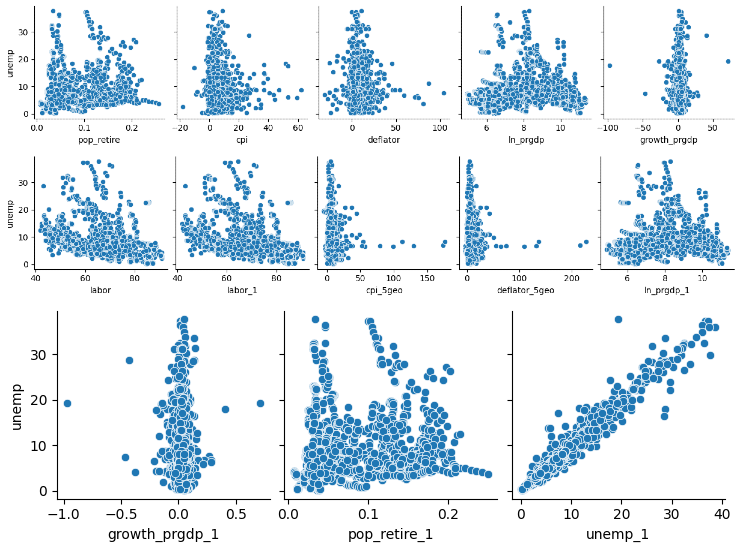
\includegraphics[width=10cm, height=8cm]{bivariate scatter total.png}
\caption{Bivariate Analysis}
\end{figure}


This can be confirmed by the correlation matrix:
\begin{figure}[h]
\centering
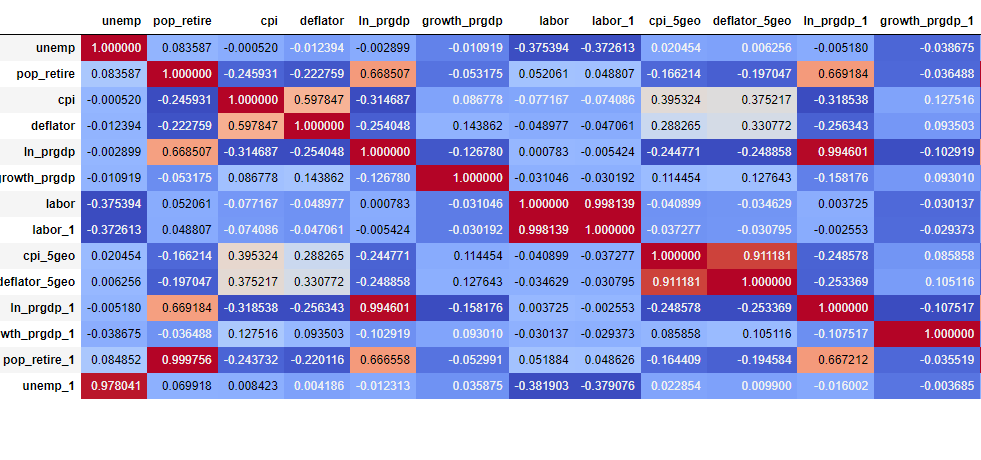
\includegraphics[width=10cm, height=8cm]{correlation matrix.png}
\caption{Correlation Matrix}
\end{figure}


Now we aim to explain how much of variance of the target variable unemployment rate could be explained by its features. After selecting eight Principal Components (PC1 to PC8), we can see that, among the 13 features ('pop\_retire', 'cpi', 'deflator','ln\_prgdp', 'growth\_prgdp', 'labor', 'labor\_1', 'cpi\_5geo', 'deflator\_5geo', 'ln\_prgdp\_1', 'growth\_prgdp\_1', 
'pop\_retire\_1', 'unemp\_1'), the first 8 features explain 96\%  and the feature of Aged Dependency Ratio played as equal important role as growth rate of per capita GDP and lagged term of unemployment rate in PC1, which accounted for 30\% variance of unemployment rate.
Therefore, the feature of old-age dependency ratio is indeed vital to for the target.

In the PCA space, the maximized variance along PC1 explains 30\% of the target, and  variable's variance. 

\subsection{Regression}

The firm plays invisible but vital role here to maintain its macroeconomic policy goals of stable product price and nonincreasing unemployment rate. It tends to provide subsidies to the firms facing falling net profit for the sake of aging. 
\fi
The regression equation is defined as:
\begin{equation} \label{eq reg}
\begin{split}
unemp_{it} &= \beta_{0}+\beta_{1}\cdot oadr+\beta_{2}\cdot oadr^2+\beta_{3}\cdot unemp\_lag+\beta_{4}\cdot labor\\
&+\beta_{5}\cdot gdppc+\beta_{6}\cdot ln\_gdppc+\beta_{7}\cdot tax\\
&+\beta_{8}\cdot gdp\_deflator+\Sigma_{j=1,j\neq t}^{62}\gamma_{j}\cdot y_{j}+u_{i}+\varepsilon_{it}
\end{split}
\end{equation}

Here the subscript $i$, $t$ refer to each country and time respectively. $u_i$ is an unobserved time-invariant random variable, which represents the intercept term of individual heterogeneity; that is, individual characteristics that do not change over time, such as the physical geography of a country, core cultural values and traditions, and historical Legacy. The composite disturbance term $u_i+\varepsilon_{it}$, $\varepsilon_{it}$ is the time-varying error term. Here the old-age dependency ratio \textbf{oadr} is the core explanatory variable, and other macroeconomic indicators such as GDP growth rate, deflator, labor participation rate, etc. are control variables. Descriptions of all variables are listed in Table~\ref{table:1}.
\begin{center}
\begin{longtable}{|m{5em}|m{6cm}|m{6cm}|}
\caption{Variable Descriptions.} \label{table:1} \\
\hline
\textbf{Variable Name} & \textbf{Economic Variable} & \textbf{Description} \\ 
\hline
\endhead % This command specifies what appears at the top of each page
\textit{unemp} & unemployment rate & \# of unemployment / (\# of unemployment + \# of employment) \\ 
\hline
\textit{oadr} & old-age dependency ratio & \# of population 65 years old and over / \# of population between 15 and 64 years old\\ 
\hline
\textit{labor} & labor participation rate & (\# of unemployment + \# of employment) / \# of population between 15 and 64 years old \\
\hline
\textit{gdppc} & gross domestic product per capita & gross domestic product / population \\
\hline
\textit{ln\_gdppc} & GDP per capita annual growth &  growth rate of gross domestic product / population\\
\hline
\textit{tax} & tax rate on income, profits and capital gains& income, profits and capital gains / total revenues \\
\hline
\textit{gdp\_deflator} & deflator &  nominal (or current-price) GDP to the real (or base year's prices) measure of GDP \\
\hline
\textit{unemp\_lag} & lag term of unemployment rate & \\
\hline
$y_{j}$ & Year dummy variable & \\
\hline
\end{longtable}
\end{center}


\section{Statistical Result Analysis}
As a benchmark, first of all, we assume there is no unobservable country-specific effect, this implies that all countries included in the dataset are assumed to share the same regression equation. Consequently, $u_{i}$ is assumed to be constant across countries in Equation \ref{eq reg} and there is no correlation within individual country groups. This means, for example, in country A, person 1 might have a high income while person 2 might have a low income, but their incomes are not related to each other. The regression results are shown in column labelled (1) in Table \ref{table:1}. The effect of the old-age dependency ratio is found to be positive. Column (2)-(4) use the equation \ref{eq reg} with the existence of $u$ assuming $\sigma_{u}\neq 0$. Specifically, column (2) represents the estimate in the presence of fixed effects (i.e. there exists correlations between the explanatory variables and the unobserved time-invariant country effect $E(x_{it},u_{i})\neq 0$). Columns (3) uses a random effects model to represent estimates conditional on the conditional expectation to zero\footnote{Please see Appendix B for the detail statistical explanation of the Pooled OLS, FE and RE FGLS.}.

\iffalse

      \hline
    $constant$ & 1.5800 & .7350\\ 
  & (.4046) & (1.0476)\\
  \hline
     &  & F Test: All $u_i=0$: \\
     &  & F(117,2061) = 2.36\\     
     &  & P-value=0.000\\ 
\hline
    $\sigma_{u}$ &  & 1.1684\\
      \hline
      $\sigma_{e} $     &  & 1.3216 \\
      \hline
      $corr(u_{i},X)$ &  & 0.6757\\
      \hline
Observation Values & 2218 & 2218\\ 
\hline

Number of Groups & 118 & 118 \\
\hline
R-Squared & 0.9342 & 0.9304 \\


\footnotetext{
In all tables here, the values in parentheses are robust standard deviations, and ***, **, and * indicate significance at the 1\%, 5\%, and 10\% confidence levels respectively. }


       &  & F test of \\
       &  & absorbed indicators:\\
       &  & F(117,2061)=2.359\\
       &  & P-value=0.000\\
       
  \hline
     &  &  \\

\hline
     &  & \\
      \hline
     &  & \\
      \hline
            $corr(u_{i},X)$ & 0 & \\
      \hline
Observation Values & 2218 & 2218 \\ 
\hline
Number of Groups & 118 & 118 \\
\hline
R Squared & 0.9420 & 0.9420\\

\fi

\begin{center}
\begin{longtable}{|m{2cm}|m{3cm}|m{3cm}|m{2.5cm}|m{3.5cm}|}
\hline
& \textbf{(1) Pooled OLS} & \textbf{(2) Fixed Effect FGLS} & \textbf{(3) Random Effect FGLS} & \textbf{(4) LSDV} \\ 

\hline
\textit{oadr} & .0402*\footnotemark & .0881* & .0560** & .0881*\\  
      &(.0218) & (.0508) & (.0229) & (.0508)\\
\hline
\textit{oadr}$^{2}$ & -.0011** & -.00259*** & -.0016** & -.00259***\\  
      & (.00054) & (.00095) & (.0006) & (.00095)\\
\hline
\textit{unemp\_lag} & .9458*** & .8505*** & .9230*** & .8505***\\  
     & (.0089) & (.0115) & (.0078) & (.0115)\\      
\hline
\textit{labor} & -.0049 & .0130 & -0.0037 & .0130\\  
     & (.0046) & (.0129) & (.0034) & (.0129)\\ 
  \hline
  \textit{gdppc} & .0000047*** & -.000001 & -.0000059** & 0.000001\\ 
  & (.0000017) & (.0000078) & (.0000028) & (.0000078)\\ 
  \hline
  \textit{ln\_gdppc} & -.1176*** & -.1202*** & -.1208*** & .1202***\\ 

  & (.02362) & (.0087) & (.0085) & (.0087)\\ 
  \hline
  \textit{tax} & -.0026 & -.0197** & -.0037 & -.0197***\\ 

  & (.0026) & (.0070) & (.0034) & (.0070)\\ 
    \hline
    \textit{gdp}\_deflator & -.0001 & .0002 & -.0001 & -.0002\\ 
  & (.0001) & (.0002) & (.0002) & (.0002\\
  \hline
    $y_{2017}$ & -.9886*** & -.6089*** & -.6219*** & -.6089***\\ 
  & (.3355) & (.2229) & (.2206) & (.2229)\\
    \hline
    $y_{2020}$ & -.5544 & -.2741 & -.2466 & -.2741\\
  & (.3800) & (.2417) & (.2426) & (.2417)\\
      \hline
    $constant$ & 1.5800 & .7350 & 1.4245 & .7350\\ 
  & (.4046) & (1.0476) & (.4474) & (1.0476)\\
  \hline
     &  & F Test: All $u_i=0$: & & F test of absorbed\\
     &  & F(117,2061) = 2.36  &  &indicators:\\     
     &  & P-value=0.000 &  & F(117,2061)=2.359\\ 
    &  & &  & P-value=0.000\\
\hline
    $\sigma_{u}$ &  & 1.1684 &  & \\
      \hline
      $\sigma_{e} $     &  & 1.3216  &  & \\
      \hline
      $corr(u_{i},X)$ &  & 0.6757 & 0 & \\
      \hline
Observation Values & 2218 & 2218 & 2218 & 2218 \\ 
\hline

Number of Groups & 118 & 118 & 118 & 118\\
\hline
R-Squared & 0.9342 & 0.9304 & 0.9420 & 0.9420\\
\hline
\end{longtable}
\end{center}

\footnotetext{
In all tables here, the values in parentheses are robust standard deviations, and ***, **, and * indicate significance at the 1\%, 5\%, and 10\% confidence levels respectively. }

It's good that the old-age dependency ratio variable is positive for Pooled OLS. But more importantly, after Pooled OLS, we have to test for the presence of an unobserved effect $u_i$ in the panel data, which reflects the heteroskedasticity across countries. If there is no such effect, then Pooled OLS is efficient and the associated statistics are asymptotically valid. Otherwise, Fixed or Random Effect models should be taken into consideration. There are 3 approaches to verify the existence of time-invariant unobserved effect $u_i$. First is the F test in column (2) of Table \ref{table:1} with the Null Hypothesis that All $u_i=0$. After estimating both models, we perform an F-test to evaluates whether the coefficients of the time-invariant variables are jointly zero. As the p-value of the F-test is 0.0000, it suggests that the Fixed Effects model is more appropriate than pooled OLS, indicating the presence of significant time-invariant omitted variables.

Second approach is the Least-squares Dummy Variable(LSDV) model, we essentially want to assess whether incorporating panel-specific effects (via dummy variables in the LSDV model) provides a better fit to the data compared to a simple pooled model. The LSDV approach is closely related to the fixed effects (FE) model and is a practical way to see the impact of omitting individual-specific effects, which takes robust standard error into account, that is, the assumption of uniform variance or homoscedasticity in a regression model is violated, this means the variance is not constant across time and countries. Here all the features have the same meaning as in \ref{eq reg} except $y_j$, which is the dummy variable taking binary values $0$ and $1$ as we take 63 years from 1960 to 2022 for each country. It turns out the coefficient of oadr from LSDV model is identical with that from fixed effect models which is shown in column 5 of Table \ref{table:1} (Due to space limitations, only part of the country dummy variables are provided). 

Breusch-Pagan Lagrange Multiplier (LM) test \cite{breusch1980lagrange} is an alternative approach to check for the presence of heteroskedasticity, i.e., whether the variance of the errors from the regression model is constant, which is statistically the same as $H_{0}: \sigma^{2}_{u}=0$. We can see the Chi-square statistic, that is, the value indicating the test statistic of the Breusch-Pagan LM test, is 1053.65, and the P-value is 0.0000, less than 1\% significance level, so we reject the Null Hypothesis of homoskedasticity (constant variance of errors), suggesting that our model's errors are heteroskedastic. The LM test result is given as in Table \ref{table:2}.


\begin{table}[t]
\centering
\caption{Breusch-Pagan Lagrange Test for Heteroskedasticity}
\label{table:2}
\begin{tabular}{lll}\toprule
%$unemp_{it} = \Sigma_{k} x_{kt}\beta_{k}+u_{i}+\varepsilon_{it},$ &t=1,..., T, i=1,..., N&\\ \midrule
Assumption: Normal error terms\\ \midrule
Variables: All independent variables\\
$H_0: \sigma^{2}_{u}=0$ \\

$\chi^{2}(01)=1053.65$\\
Prob $> \chi^{2} = 0.0000$\\ \bottomrule
	\end{tabular}
\end{table}


\iffalse
Assumption: Normal error terms
Variables: All independent variables

H0: Constant variance

   chi2(39) = 1053.65
Prob > chi2 =  0.0000
\fi



It turns out the P-value is 0.0000, which means the Null Hypothesis should be rejected. Therefore, there exists unobserved effect and the Random or Fixed Effect models are more appropriate than Pooled OLS. This can also be confirmed by the F test in column (2) of table \ref{table:1} which tests whether there are omitted variables that do not change over time, with the Null Hypothesis of "$H_0$: All $u_i=0$". The P-value of the F test is 0.0000, so we reject the Null Hypothesis, that is, the fixed effects model is superior than the Pooled regression. It can also be seen from table \ref{table:2} that individual country dummy variable is significant for most of countries, which means there exist individual effects. Therefore, Pooled regression should not be used. From Random and Fixed Effect models, it's clear that the impact of old-age dependency ratio on unemployment is positive and large, and the estimator is highly statistically significant.

In summary, after adjusting for the influence of time and other key macroeconomic variables traditionally considered to influence the unemployment rate, through the application of Pooled OLS, Fixed Effect, and Random Effect Feasible Generalized Least Squares, we discovered that the relationship between the unemployment rate ($r_u$ in short) and the old-age dependency ratio ($oadr$ in short) appears to in quadratic form. Specifically, The formula is expressed as 
$r_u = a\cdot oadr^2 + b\cdot oadr + c$, where $a<0$ and $b>0$. Given that the calculated axis of symmetry, determined by $-\frac{b}{2a}$, surpasses 40 in all four models --- far exceeding the real-world old-age dependency ratios, such as Japan's 0.51 in 2022 --- the portion of the curve of interest is the ascending segment to the left of the axis of symmetry. 
Furthermore, we employed three different methods to test the existence of heteroskedasticity across countries. These tests reveal that the outcomes derived from either the Fixed Effect or Random Effect models are more reliable than those obtained from the Pooled OLS ones.
Finally, these results confirm a positive impact of the old-age dependency ratio on the unemployment rate in real-world data, which aligns with the findings from our agent-based model.
%This finding underscores the importance of accounting for unobserved heterogeneity when analyzing the dynamics between the old-age dependency ratio and unemployment rates.

\chapter{Conclusions}
\section{Main Conclusions}
In conclusion, this paper sheds light on the dynamics between aging populations and labor markets, particularly highlighting the impact on goods prices adjustment. Through empirical observations and the development of a search and matching model and an agent-based model, we unveil the dual effects of aging: while retirees contribute to increased net demand, fostering employment opportunities, their distinct price sensitivity poses challenges for manufacturers, leading to competitive pricing strategies. Our study shows that changes due to more older people can lead to businesses making less money and more people being out of work. This key finding points out how changes in the population and the economy are connected. It suggests we need to think again about how we approach market strategies and policies. This interplay between demand stimulation and price pressure underscores the complexity of the relationship between aging and key economic indicators, offering valuable insights for policymakers and stakeholders navigating the evolving landscape of labor markets in aging societies.
% Show layout for debug purposes 
%    \layout
\section{Limitations and Future Work}
While the models presented in this thesis provide valuable insights into the interplay between an aging population, labor markets, and pricing dynamics, there are several limitations that should be acknowledged and addressed in future research.
First, the current analysis does not explicitly account for the heterogeneity within the retired population, particularly those who live in poverty. This oversight is especially relevant in regions such as sub-Saharan Africa and certain countries like China and South Korea, where government support for the elderly is limited. Future work should incorporate the economic circumstances of impoverished retirees, as their consumption patterns and price sensitivity may differ significantly from their more financially secure counterparts.
Second, the mathematical models employed in this thesis assume constant birth and mortality rates, which oversimplifies the dynamic nature of population changes. Future iterations of the models should incorporate time-varying birth and mortality rates to better reflect real-world demographic shifts and their potential impact on labor markets and pricing dynamics.
Third, the current analysis primarily relies on empirical observations from different countries, which may not fully capture the nuances and intricacies of each nation's unique economic and societal landscape. Future research could focus on developing country-specific models that account for cultural, institutional, and policy factors that may influence the relationship between aging populations, labor markets, and pricing.

\appendix
\setcounter{section}{0}
\renewcommand{\thesection}{\Alph{section}}
\section{Appendix: Proof of Lemma \ref{Lemma}}
\begin{proof}
Under conditions of perfect market competition, assuming seller A offers a price $p>\bar{p}>c$, because buyers have the possibility of conducting secondary searches, seller B only needs to choose a price 
$p-\epsilon\geq\bar{p}$, where $\epsilon>0$, to capture all consumers and still remain profitable. Considering that all sellers understand this, the final equilibrium price $p$ should satisfy $p\leq\bar{p}$.
\qed
\end{proof}
\section{Appendix: Economic Terminology Explanations}
\subsection{Introduction to Panel Data Analysis Methods}
The following discussion are mainly from the text of \cite{wooldridge2010econometric}, with the exception of the detailed mathematical derivation.

Panel data, also known as longitudinal or cross-sectional time-series data, provide valuable insights into economic phenomena by capturing observations across multiple entities over time. In this Appendix, we introduce three common methods for analyzing panel data: pooled ordinary least squares (POLS), random effects, and fixed effects generalized least squares (GLS).

The Pooled OLS model employs the Ordinary Least Squares (OLS) approach to analyze panel data, and treats all countries and time periods equally, assuming constant coefficients. That is, under Equation \ref{eq reg}, the parameter $u_i$ is considered to be constant across countries, and there is no interdependence observed within individual countries. Therefore, we can rewrite Equation \ref{eq reg} in simple form as 
\begin{equation} \label{eq simple reg}
y_{it}=\beta_{0}+x_{it}\beta_{1}+\varepsilon_{it}, t = 1,2, ..., T, i = 1, 2, ..., N.
\end{equation}
To consistently estimate the coefficient $\beta$, three assumptions are usually sufficient:\\
\noindent \textbf{Assumption POLS.1:} Exogeneity: The independent variable $x_{it}$ is uncorrelated with the error term $\varepsilon_{it}$:
$\textbf{E}(\varepsilon_{it}|x_{it})=0,  t = 1,2, ..., T.$

\noindent \textbf{Assumption POLS.2:} Independence and Identically Distributed (i.i.d): Independent variables $x_{it}$ are i.i.d across countries: 
\iffalse $\textbf{rank} [\sum_{t=1}^{T}\textbf{E}(X^{T}_{t} X_t)]=6,  t = 1,2, ..., T.$ \fi

\noindent \textbf{Assumption POLS.3:} Homoscedasticity: The error term $\varepsilon_{it}$ has constant variance across all countries and over time.

(a) $\textbf{E}(\varepsilon_{it}^{2}|x_{it})=\sigma^2,  t = 1,2, ..., T, i = 1,2,..., N;$

(b) $\textbf{E}(\varepsilon_{it}\varepsilon_{is}|x_{it}, x_{is})=0, t\neq s, t, s = 1,..., T, i = 1,2,..., N.$

\noindent Here \textbf{Assumption POLS.3} guarantees a homoskedasticity variance matrix. 
But based on the results of the LM test as well as F test we've done in Section 5, this assumption could not hold as there exists an unobserved effect across countries, which means the existence of either heteroskedasticity: $\textbf{Var}(\varepsilon|X)=\Omega \neq \sigma^{2}I_n$ or serial correlation: $Cov(\varepsilon_{t}\varepsilon_{s}|X_{t}, X_{s})\neq 0)$.
To ensure the estimators are efficient, we transform the model \ref{eq simple reg} by left multiplying $\textbf{w}$ on both sides, 
$$\textbf{w}y_{t} = \textbf{w}X_t\beta+\textbf{w}\varepsilon_{t}$$ where $
\textbf{w}$ satisfies $\textbf{w}^{T}\textbf{w}=\Omega^{-1}$, a \textbf{Cholesky decomposition} of $\Omega^{-1}$. An issue arises here as it's hard to know the matrix $\Omega$, let alone determine its singularity and compute its inverse if it's nonsingular. So here is the trick of Feasible Generalized Least-square method. 
\begin{enumerate}
  \item Pooled OLS is applied to the data, and then residuals ($\hat{\varepsilon_t}$) are computed.
  \item Variance matrix $\hat{\Omega}=var(\hat{\varepsilon_t})$ is estimated based on the Pooled model (Here explains the meaning of "feasible").
  \item The coefficient $\hat{\beta}_{FGLS}$ is estimated as $(X^{T}\hat{\Omega}^{-1}X)^{-1}(X^{T}\hat{\Omega}^{-1}y)$ along with its covariance matrix.
  \item This process can be iterated until $\hat{\beta}_{FGLS}$ converges.
\end{enumerate}

One significant advantage of fixed or random effect FGLS models is their ability to account for all time-invariant unmeasured (or latent) variables that impact the dependent variable, that is, $u_i$ in Equation \ref{eq reg}, regardless of whether these factors are recognized or not by the researcher. This is particularly valuable given the probable existence of these unaccounted variables. The Random Effects Model assumes that these unobserved, time-invariant variables do not have any correlation with the included time-varying variables~\cite{wooldridge2010econometric}, that is, $\textbf{cov}(x_{it}, u_i)=0$ where $x_{it}$ means all the explanatory variables in Equation \ref{eq reg} including oadr, labor, etc. On the other hand, the Fixed Effects Model (FEM) permits these variables to exhibit correlations.
\subsection{Least-squares Dummy Variable (LSDV)}
The Least-squares Dummy Variable model is actually the Ordinary Least-squares approach with addition of dummy variables. It has the advantage that we don't need to adjust the variance matrix, just like what we have done in Feasible Generalized Least-squares (FGLS). The result from LSDV estimation is equvalent to Fixed-effects within group FGLS, which you can see from column 3 of Table \ref{table:1} and Table \ref{table:2}.


\section{Appendix: Newton-Raphson Method}
\subsection{Mathematical Principal}
Our system consists of 4 variables ($u, \theta, \pi, p$) and 4 equations:
%\begin{enumerate}
   \begin{equation}
   q(\theta)(1-\phi)(y(p-c)-y_u)-c = 0
   \end{equation}

   \begin{equation} \label{eq12}
\begin{split}
&\frac{(n-u)(1+\psi_e)}{b}(1-\frac{2\psi_e}{1+\psi_e}\nu)\frac{w_{op}(u,a)}{p}(p-c)+\frac{u(1+\psi_u)}{b}(1-\frac{2\psi_u}{1+\psi_u}\nu)\frac{y_u}{p}(p-c)\\
&+\frac{a(1+\psi_a)}{b}(1-\frac{2\psi_a}{1+\psi_a}\nu)\frac{y_a}{p}(p-c)-m(u,v)y(p-c)=0
\end{split}
\end{equation}

   \begin{equation}
    m(u,v)w+\pi-m(u,v)y(p-c)=0
   \end{equation}

   \begin{equation}   
    (n-u)\delta-uf(\theta) = 0
   \end{equation}
with $w_{op}(u,a)=(1-\phi)y_u+\phi y(p-c)$ in Equation \ref{eq12}. This is equivalent to finding the zeroes of a single vector-valued function $F: \mathbb{R}^4\rightarrow \mathbb{R}^4$, with $$
F = \begin{pmatrix}
F_{1}\\
F_{2}\\
F_{3}\\
F_{4}\\
\end{pmatrix}=\begin{pmatrix}
q(\theta)(1-\phi)(y(p-c)-y_u)-c\\
\begin{split}
&\frac{(n-u)(1+\psi_e)}{b}(1-\frac{2\psi_e}{1+\psi_e}\nu)\frac{w_{op}(u,a)}{p}(p-c)+\frac{u(1+\psi_u)}{b}(1-\frac{2\psi_u}{1+\psi_u}\nu)\frac{y_u}{p}(p-c)\\
&+\frac{a(1+\psi_a)}{b}(1-\frac{2\psi_a}{1+\psi_a}\nu)\frac{y_a}{p}(p-c)-m(u,v)y(p-c)
\end{split}\\
m(u,v)w+\pi-m(u,v)y(p-c)\\
(n-u)\delta-uf(\theta)
\end{pmatrix}$$ where the independent vector variable is $x=(u, \theta, \pi, p)$. Newton-Raphson method starts with an initial guess of $x_0$ for the root of $F$, if first-order partial derivatives of $F$ with respect to $x$ exist and the initial guess is luckily close, then
$$x_{n+1}=x_{n} - J_{F}(x_{n})^{-1}F(x_{n})$$
where $J_{F}(x_{n})$ is the $4\times4$ Jacobian matrix of function $F$:
$$F=\begin{pmatrix}
    \frac{\partial F_1}{\partial u}  & \dots & \frac{\partial F_1}{\partial u}\\
    \vdots & \ddots & \vdots\\
    \frac{\partial F_4}{\partial p}  & \dots & \frac{\partial F_1}{\partial p}
\end{pmatrix}$$

To save time and increase numerical stability, one may avoid computing the inverse of the Jacobian matrix, rather, sovle the following linear equations for $x_{n+1}$
$$J_{F}(x_{n})(x_{n+1} - x_{n}) = - F(x_{n})$$
with $x_0$ given.
We depict the process of locating the root $x_n$ of the system in Figure \ref{figNR}, specifically in the context of a single-variable, single-equation scenario\footnote{Figure Source: https://en.wikipedia.org/wiki/Newton\%27s\_method}.
\begin{figure}[h]
\centering
\includegraphics[width=10cm, height=8cm]{Newton_iteration.svg.png}
\caption{Process of finding a better approximation for the root $x$ of the function $f$}
\label{figNR}
\end{figure}

\iffalse
\subsection{Code}
\begin{lstlisting}[language=Python, caption=Newton Raphson Method]
import sys, numpy as np, matplotlib.pyplot as plt

s = 0.6 # the bargaining power of the workers
psi_e = 0
psi_u = 0.5
psi_a = 1
n = 1
y_u = 0.4
y_a = 0.4
bar_p = 1
y = 1
c = 0.1
delta = 0.1

# let the matching function in labor market
# m(u,v)=kappa*u**zeta*v**(1-zeta)
# then q(theta) = m(u,v)/v = kappa*theta**(-zeta),f(theta) = m(u,v)/u = kappa*theta**(1-zeta)

kappa = 0.5
zeta = 0.35

'''
q = kappa* (theta) ** (-zeta)
f = theta*q
b = (n-u)*(1+psi_e)+u*(1+psi_u)+a*(1+psi_a)
w = (1-s)*y_u + s*pi

'''

# x = (u, theta, p)
# profit = m(u,v)y*(p-c)-m(u,v)*w

def func1(x):
# use np.sign(a)*(np.abs(a))**(-zeta) to avoid Numpy not allowing fractional powers of negative numbers

    return c-kappa*np.sign(x[1])*(np.abs(x[1]))**(-zeta)*(1-s)*(y*(x[2]-c)-y_u)

def func2(x):
    b = (n-x[0])*(1+psi_e)+x[0]*(1+psi_u)+a*(1+psi_a)
    w = (1-s)*y_u + s*y*(x[2]-c)
    m = kappa*x[0]**zeta*(x[0]*x[1])**(1-zeta)

    return (n-x[0])*(1+psi_e)/b*(1-2*psi_e/(1+psi_e)*(n-x[0]-a)/b)*w/x[2]*(x[2]-c)\
+x[0]*(1+psi_u)/b*(1-2*psi_u/(1+psi_u)*x[0]/b)*y_u/x[2]*(x[2]-c)\
+a*(1+psi_a)/b*(1-2*psi_a/(1+psi_a)*a/b)*y_a/x[2]*(x[2]-c)-m*y*(x[2]-c)+m*w

def func3(x):
    return x[0]*kappa*np.sign(x[1])*(np.abs(x[1]))**(1-zeta)-(n-x[0])*delta

func = [func1, func2, func3]

from autograd import grad, jacobian

a = 0.5

x = np.array([0.01,1,0.1], dtype=float)
x_0 = x.copy()

grad_func0 = grad(func1)
grad_func1 = grad(func2)
grad_func2 = grad(func3)

jacobi = [grad_func0(x), grad_func1(x), grad_func2(x)]

x_1 = x_0 - np.matmul(np.linalg.inv(jacobi),[func1(x_0), func2(x_0), func3(x_0)])
error = np.linalg.norm(x_1-x_0)

iteration = 0
maxiteration = 10**2
threshold = 10**(-2)
t_0 = np.array([0.1, 0.5, 1], dtype=float)

while error > threshold and (iteration < maxiteration):
    iteration += 1
    t_1 = t_0 - np.matmul(np.linalg.inv(jacobi),[func1(t_0), func2(t_0), func3(t_0)])
    error = np.linalg.norm(t_1-t_0)
    t_0 = t_1
    print("x[", iteration, ']=', t_0 )
\end{lstlisting}
\fi

To test the correctness of algorithm, we tried a simple 2-variable 2-equations system, which we have known the solution beforehand, The output of the Newton-Raphson method turns out to be convergent as belows.
\begin{lstlisting}
x[ 1 ]= [0.8  0.88]
x[ 2 ]= [0.94144  0.956096]
x[ 3 ]= [0.98004288 0.98406316]
x[ 4 ]= [0.99288644 0.99419407]
x[ 5 ]= [0.99742453 0.99788152]
\end{lstlisting}
However, while solving the 4-variable, 4-equation system, the output is divergent:
\begin{lstlisting}
x[ 1 ]= [0.19491469 0.86528246 0.81158014]
x[ 2 ]= [0.16858801 3.20240073 0.65661713]
x[ 3 ]= [-0.01263441  6.97291132  0.52453244]
x[ 4 ]= [nan nan nan]
\end{lstlisting}
The Newton-Raphson method failed to converge for the system primarily due to the initial value of $x_0$. Despite attempting various values, the output remained non-convergent.
    % Bibliography
    \bibliographystyle{unsrt}
    \bibliographystyle{plainnat}
    \bibliography{test-bib}

\end{document}
